% !TEX root = saveliev_physics_general_course_1.tex
%!TEX TS-program = pdflatex
%!TEX encoding = UTF-8 Unicode


\chapter{KINEMATICS}\label{chap:1}

\section{Mechanical motion}\label{sec:1_1}

Mechanical motion is the simplest form of motion of matter. It consists in the movement of bodies or their parts relative to one another. We can see movements of bodies everywhere in our ordinary life. This is why mechanical notions are so clear. This also explains the fact that mechanics was the first of all the natural sciences to be developed very broadly.

A combination of bodies separated for consideration is called a \textbf{mechanical system}. The bodies to be included in a system depend on the nature of the problem being solved. In a particular case, a system may consist of a single body.

It was indicated above that motion in mechanics is defined as the change in the mutual arrangement of bodies. If we imagine a separate isolated body in a space where no other bodies are present, then we cannot speak of the motion of the body because there is nothing with respect to which the body could change its position. It thus follows that if we intend to study the motion of a body, then we must indicate with respect to what other bodies the given motion occurs.

Motion occurs both in space and in time (space and time are inalienable forms of existence of matter). Consequently, to describe motion, we must also determine time. We use a timepiece (watch or clock) for this purpose.

A combination of bodies that are stationary relative to one another with respect to which motion is being considered and a timepiece indicating the time forms a \textbf{reference frame}.

The motion of the same body relative to different reference frames may have a different nature. For example, let us imagine a train gaining speed. Suppose that a passenger is walking with a constant velocity along the corridor of one of the cars of the train. The motion of the passenger relative to the ear will be uniform, and relative to the Earth's surface it will be accelerated.

To describe the motion of a body means to indicate for every moment of time the position of the body in space and its velocity. To set the state of a mechanical system, we must indicate the positions and the velocities of all the bodies forming the system. A typical problem of mechanics consists in determining the states of a system at all the following moments of time $t$ when we know the state of the system at a certain initial moment $t_0$ and also the laws governing the motion.

It must be noted that no physical problem can be solved absolutely exactly. An approximate solution is always obtained. The degree of approximation is determined by the nature of the problem and the object to be achieved. In solving a problem approximately, we disregard the factors that are not significant in the given case. For example, we may often disregard the dimensions of the body whose motion is being studied. For instance, it is quite possible to disregard the Earth's dimensions when treating its motion about the Sun. This allows us to considerably simplify our description of the motion because the Earth's position in space can be determined by a single point.

A body whose dimensions may be disregarded in the conditions of a given problem is called a \textbf{point particle} (or simply a \textbf{particle}). Whether or not we may consider a given body as a particle depends not on the dimensions of the body, but on the conditions of the problem. The same body in some cases may be treated as a particle, but in others it must be considered as an extended body.

When speaking about a body as a particle, we disengage ourselves from its dimensions. Another abstraction which we have to do with in mechanics is a perfectly rigid body. Absolutely undeformable bodies do not exist in nature. Any body deforms to a greater or smaller extent, \ie, changes its shape and dimensions, under the action of forces applied to it. The deformations of bodies when considering their movements may often be disregarded, however. If this is done, then the body is called perfectly rigid. Thus, a body whose deformations may be disregarded in the conditions of a given problem is called a \textbf{perfectly rigid}, or simply a \textbf{rigid body}.

Any motion of a rigid body can be resolved into two basic kinds of motion---\textbf{transla\-tional motion} and \textbf{circular motion}.

Translational motion (translation) is defined as motion in which any straight line associated with the moving body remains parallel to itself (\fig{1_1}).

In circular motion (rotation), all the points of a body move in circles whose centers are on a single straight line called the axis of rotation (\fig{1_2}). The axis of rotation can be outside a body (see \fig{1_2}b).

\begin{figure}[t]
	\begin{minipage}[t]{0.5\linewidth}
		\begin{center}
			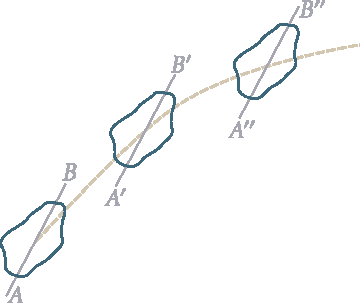
\includegraphics[scale=0.95]{figures/ch_01/fig_1_1.pdf}
			\caption[]{}
			\label{fig:1_1}
		\end{center}
	\end{minipage}
	\hfill{ }%\hspace{-0.1cm}
	\begin{minipage}[t]{0.5\linewidth}
		\begin{center}
			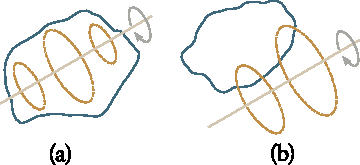
\includegraphics[scale=0.95]{figures/ch_01/fig_1_2.pdf}
			\caption[]{}
			\label{fig:1_2}
		\end{center}
	\end{minipage}
%\vspace{-0.5cm}
\end{figure}

\begin{figure}[t]
	\begin{center}
		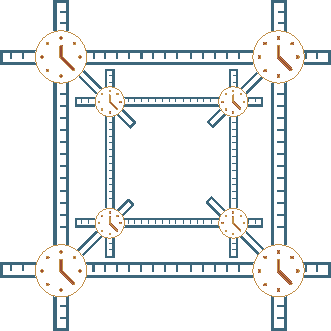
\includegraphics[scale=0.95]{figures/ch_01/fig_1_3.pdf}
		\caption[]{}
		\label{fig:1_3}
	\end{center}
	\vspace{-0.8cm}
\end{figure}

Since when treating a body as a particle we ignore its length, the concept of circular motion about an axis passing through such a body cannot be applied to it.

To acquire the possibility of describing motion quantitatively, we have to associate a \textbf{coordinate system} (for example a Cartesian one) with the bodies forming a reference frame. Hence, the position of a particle can be determined by setting the three numbers $x$, $y$, and $z$---the Cartesian coordinates of the particle. A coordinate system can be made by forming a rectangular lattice from identical rods or rules graduated to a definite scale: (\fig{1_3}). Identical clocks synchronized with one another must be placed at the lattice points. The position of a particle and the moment of time corresponding to this position are recorded on the graduated rods and the clock closest to the particle.

It is simpler to treat a point particle than an extended body. We shall therefore first study the mechanics of a particle, and then go over to the mechanics of a rigid body. We shall start with kinematics, and then delve into dynamics. We remind our reader that \textbf{kinematics} studies the motion of bodies without regard to what causes this motion. \textbf{Dynamics} studies the motion of bodies with a view to what causes this motion to have the nature it does, \ie, with a view to the interactions between bodies.

\section{Vectors}\label{sec:1_2}

\textbf{Definition of a Vector.} Vectors are defined as quantities characterized by a numerical value and a direction and also as ones that are added according to the triangle or parallelogram method\footnote{According to a stricter definition, a vector is a combination of three quantities that transform when the coordinate axes rotate according to a definite law.}. The last requirement is a very significant one. We can indicate quantities characterized by a numerical value and a sense of direction but that are added in a different way than vectors. We shall take as an example the rotation of a body about an axis through the finite angle $\varphi$. Such rotation can be depicted in the form of a segment of length $\varphi$ directed along the axis about which rotation is occurring and pointing in a direction associated with that of rotation according to the right-hand screw rule. The top portion of \fig{1_4} shows two consecutive turns of the sphere through the angles $\pi/2$ depicted by the segments $\varphi_1$ and $\varphi_2$. The first turn about axis $1$---$1$ transfers point $A$ of the sphere to position $A'$, and the second turn about axis $2$---$2$ transfers it to position $A''$. The same result, \ie, transfer of point $A$ to position $A''$, can be achieved by turning the sphere about axis $3$---$3$ (see the bottom portion of \fig{1_4}) through the angle $\pi$. Hence, such a turn should be considered as the sum of the turns $\varphi_1$ and $\varphi_2$. It cannot be obtained from the segments $\varphi_1$ and $\varphi_2$, however, by adding them according to the parallelogram method. Such addition gives a segment of length $\pi/\sqrt{2}$ instead of the required length $\pi$. Rotation through the angle $\pi/\sqrt{2}$ transfers point $A$ to point $A'''$. It thus follows that the turns through finite angles depicted by the directed segments do not have the properties of vectors.

\begin{figure}[t]
	\begin{center}
		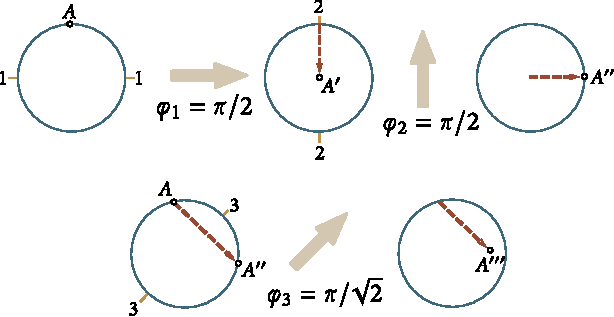
\includegraphics[scale=0.9]{figures/ch_01/fig_1_4.pdf}
		\caption[]{}
		\label{fig:1_4}
	\end{center}
\vspace{-0.8cm}
\end{figure}

The numerical value of a vector is called its magnitude. Figuratively speaking, the magnitude of a vector indicates its length. The magnitude of a vector is a scalar, and always a positive one.

Vectors are represented graphically by arrows. The length of an arrow determines to the established scale the magnitude of the relevant vector, and the arrow points in the direction of the vector.

Vectors are customarily distinguished by setting their symbols in boldface type, for example, $\vec{a}$, $\vec{b}$, $\vec{v}$ and $\vec{F}$. The same symbols set in italics signify the magnitude of the relevant vectors, for example, $a$ is the magnitude of the vector $\vec{a}$\footnote{In handwriting, vectors are denoted by arrows over their symbols (for example, $\oldvec{a}$. In this case, the same letter without the arrow stands for the magnitude of the vector.}. It is sometimes necessary to express the magnitude by placing a vertical bar (an absolute value sign) on each side of the symbol for the vector. Thus, $|a|$ is the magnitude of the vector $\vec{a}$. This representation is used, for example, to show the magnitude of the sum of the vectors $\vec{a}_1$ and $\vec{a}_2$:
\begin{equation}\label{eq:1_1}
	|\vec{a}_1 + \vec{a}_2| = \text{magnitude of the vector } (\vec{a}_1 + \vec{a}_2).
\end{equation}

\noindent
In this case, the notation $a_1+a_2$ signifies the sum of the magnitudes of the vectors being added, which in general does not equal the magnitude of the sum of the vectors (the two sums will be equal only when the vectors being added have the same direction).

Vectors directed along parallel straight lines (in the same or in opposite directions) are called \textbf{collinear}. Vectors in parallel planes are called \textbf{coplanar}. Collinear vectors can be arranged along the same straight line and coplanar vectors can be brought into one plane by parallel translation.

Collinear vectors equal in magnitude and having the same direction are considered to equal each other\footnote{What is meant are the so-called \textbf{free vectors}, \ie, vectors that can be drawn from any point in space. Also distinguished are \textbf{slip vectors} whose tail can be placed at any point on the straight line along which the vector is directed, and localized vectors, which are applied to a definite point. The last two kinds of vectors can be expressed through free vectors. This is why vector calculus is based on the concept of the free vector, usually called simply a vector.}.

\textbf{Vector Addition and Subtraction.} It is more convenient to add vectors in practice without constructing a parallelogram. Examination of \fig{1_5} shows that we can achieve the same result if we bring the tail of the second vector in contact with the tip of the first one, and then draw the resultant vector from the tail of the first vector to the tip of the second one. It is very good to use this procedure when we have to add more than two vectors (\fig{1_6}).

\begin{figure}[t]
	\begin{minipage}[t]{0.5\linewidth}
		\begin{center}
			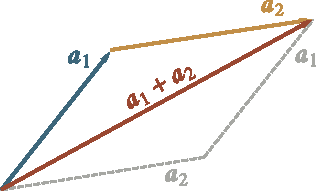
\includegraphics[scale=0.95]{figures/ch_01/fig_1_5.pdf}
			\caption[]{}
			\label{fig:1_5}
		\end{center}
	\end{minipage}
	\hfill{ }%\hspace{-0.1cm}
	\begin{minipage}[t]{0.5\linewidth}
		\begin{center}
			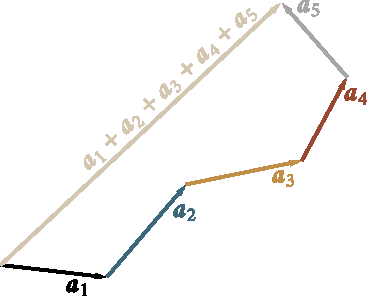
\includegraphics[scale=0.95]{figures/ch_01/fig_1_6.pdf}
			\caption[]{}
			\label{fig:1_6}
		\end{center}
	\end{minipage}
\vspace{-0.7cm}
\end{figure}

The difference of two vectors $\vec{a}$ and $\vec{b}$ is defined as such a vector $\vec{c}$ which when added to the vector $\vec{b}$ gives the vector $\vec{a}$ (\fig{1_7}---the vector $-\vec{b}$ depicted by a dash line will be treated below The magnitude of the difference of two vectors, like the magnitude of a sum [see \eqn{1_1}], may be written only with the aid of vertical bars:
\vspace{-12pt}
\begin{equation}\label{eq:1_2}
|\vec{a}_1 - \vec{a}_2| = \text{magnitude of the vector } (\vec{a}_1 - \vec{a}_2),
\end{equation}

\noindent
because the notation $a_1-a_2$ signifies the difference of the magnitudes of the vectors $\vec{a}_1$ and $\vec{a}_2$, which, generally speaking, does not equal the magnitude of the vector difference.

\textbf{Multiplication of a Vector by a Scalar.} Multiplication of the vector $\vec{a}$ by the scalar $\alpha$ yields a new vector $\vec{b}=\alpha\,\vec{a}$ whose magnitude is $|\alpha|$ times that of the vector a (\ie, $b=|\alpha|a$). The direction of the vector $\vec{b}$ either coincides with that of the vector $\vec{a}$ (if $\alpha>0$), or is opposite to it (if $\alpha<0$). It follows from the above that multiplication by $-1$ reverses the direction of a vector. Consequently, the vectors $\vec{a}$ and $-\vec{a}$ have the same magnitudes, but are opposite in direction. It is simple to see with the aid of  \fig{1_7} that subtraction of the vector $\vec{b}$ from the vector $\vec{a}$ is equivalent to addition of the vector $-\vec{b}$ to the vector $\vec{a}$.

It follows from our definition of multiplication of a vector by a scalar that any vector $\vec{a}$ can be represented in the form
\begin{equation}\label{eq:1_3}
\vec{a} = a\,\vecuni{a},
\end{equation}

\noindent
where $a$ is the magnitude of the vector $\vec{a}$ and $\vecuni{a}$, is vector with a magnitude of unity and of the same direction as $\vec{a}$ (\fig{1_8}).

The vector $\vecuni{a}$ is called the unit vector of the vector $\vec{a}$. The unit vector can be represented in the form
\begin{equation}\label{eq:1_4}
\vecuni{a} = \frac{\vec{a}}{a},
\end{equation}

\noindent
whence it follows that it is a dimensionless quantity.

\begin{figure}[t]
	\begin{minipage}[t]{0.5\linewidth}
		\begin{center}
			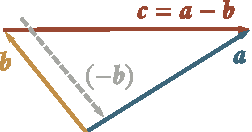
\includegraphics[scale=0.9]{figures/ch_01/fig_1_7.pdf}
			\caption[]{}
			\label{fig:1_7}
		\end{center}
	\end{minipage}
	\hfill{ }%\hspace{-0.1cm}
	\begin{minipage}[t]{0.5\linewidth}
		\begin{center}
			
\includegraphics[scale=0.95]{figures/ch_01/fig_1_8.pdf}
			\caption[]{}
			\label{fig:1_8}
		\end{center}
	\end{minipage}
\vspace{-0.6cm}
\end{figure}

Unit vectors can be compared not only with vectors, but also with any direction in space. For example, $\vecuni{x}$ is the unit vector of the coordinate axis $x$, $\vecuni{n}$ is the unit vector of a normal to a curve or surface, and $\vecuni{\tau}$ is the unit vector of a tangent to a curve.

\textbf{Linear Relation Between Vectors.} Let us consider three non-collinear vectors $\vec{a}$, $\vec{b}$ and $\vec{c}$ that are in one plane. A glance at \fig{1_9} shows that any of them (for instance, $\vec{c}$) can be expressed through the other two with the aid of the relation
\begin{equation}\label{eq:1_5}
\vec{c} = \alpha\vec{a} + \beta\vec{b},
\end{equation}

\noindent
where $\alpha$ and $\beta$ are scalars (for the case shown in the figure, $\alpha>1$ and $-1<\beta<0$). Hence, we conclude that any vector $\vec{c}$ that is in the same plane as the non-collinear vectors $\vec{a}$ and $\vec{b}$ can be expressed through the latter with the aid of linear relation~\eqref{eq:1_5}. When the vectors $\vec{a}$ and $\vec{b}$ are fixed, any third vector is unambiguously determined by the two quantities $\alpha$ and $\beta$.

Assume that we have three vectors $\vec{a}$, $\vec{b}$ and $\vec{c}$, each of which is not coplanar with the other two.\footnote{Two vectors are always coplanar. This follows from the fact that their tails can he made to coincide by translation, and they will thus be in one plane.} By analogy with \eqn{1_5}, we can see quite easily that any vector $\vec{d}$ can be represented as a linear combination of the given vectors:
\begin{equation}\label{eq:1_6}
\vec{d} = \alpha\vec{a} + \beta\vec{b} + \gamma\vec{c},
\end{equation}

\noindent
When the vectors $\vec{a}$, $\vec{b}$ and $\vec{c}$ are fixed, any vector $\vec{d}$ is unambiguously determined by the three quantities $\alpha$, $\beta$ and $\gamma$, each of which may be either positive or negative.

\textbf{Projection of a Vector.} Let us consider a direction in space that we shall set by the axis $l$ (\fig{1_10}). Let the vector $\vec{a}$ make the angle $\varphi$ with the axis $l$\footnote{If the straight line along which the vector $\vec{a}$ is directed and the axis $l$ do not intersect, the angle $\varphi$ should be found by drawing a straight line parallel to the vector $\vec{a}$ and intersecting the axis $l$. The angle between this line and the axis $l$ will be the angle $\varphi$ we are interested in.}. The quantity
\begin{equation}\label{eq:1_7}
a_l = a\, \cos\varphi
\end{equation}

\noindent
(where $a$ is the magnitude of the vector) is called the projection of the vector $\vec{a}$ onto the axis$l$. A projection is designated by the same symbol as its vector, with the addition of a subscript showing the direction onto which the vector has been projected.

\begin{figure}[t]
	\begin{minipage}[t]{0.5\linewidth}
		\begin{center}
			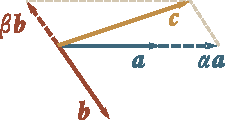
\includegraphics[scale=1]{figures/ch_01/fig_1_9.pdf}
			\caption[]{}
			\label{fig:1_9}
		\end{center}
	\end{minipage}
	\hfill{ }%\hspace{-0.1cm}
	\begin{minipage}[t]{0.5\linewidth}
		\begin{center}
			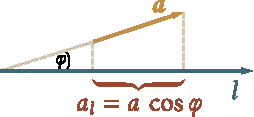
\includegraphics[scale=0.95]{figures/ch_01/fig_1_10.pdf}
			\caption[]{}
			\label{fig:1_10}
		\end{center}
	\end{minipage}
	\vspace{-0.7cm}
\end{figure}

A projection of a vector is an algebraic quantity. If the vector makes an acute angle with the given direction, then $\cos\varphi>0$, and the projection is positive. If the angle $\varphi$ is obtuse, then $\cos\varphi<0$, and, consequently, the projection is negative. When a vector is at right angles to a given axis, its projection equals zero.

The projection of a vector has a simple geometrical meaning. It equals the distance between the projections of the tail and the tip of the segment depicting the given vector onto the given axis. When $\varphi<\pi/2$, this distance is assumed to be positive, and when $\varphi>\pi/2$, it is negative.

Let $\vec{a} = \vec{a}_1+\vec{a}_2+\vec{a}_3+\vec{a}_4$ (\fig{1_11}). It is easy to see from the figure that the projection of the resultant vector a onto a direction $l$ equals the sum of the projections of the separate vectors being added:
\begin{equation}\label{eq:1_8}
a_l = a_{1l}+a_{2l}+a_{3l}+a_{4l}.
\end{equation}

\noindent
We must remind our reader that when adding the projections of the vectors shown in \fig{1_11}, the distances $0$---$1$, $1$---$2$, and $2$---$3$ have to be taken with the plus sign, and the distance $3$---$4$ with the minus sign. Equation~\eqref{eq:1_8} holds for any number of addends.

\textbf{Expressing a Vector Through Its Projections onto the Coordinate Axes.} Let us take Cartesian coordinate axes and consider the vector $\vec{a}$ in a plane at right angles to the $z$-axis (\fig{1_12}). We shall introduce the unit vectors of the coordinate axes, \ie, the unit vectors $\vecuni{x}$, $\vecuni{y}$ and $\vecuni{z}$ ($\vecuni{z}$ is not shown in the drawing, it is perpendicular to the plane of the drawing and directed toward us). It must be noted that these three unit vectors completely determine a system of coordinates and are therefore called the \textbf{basis of the coordinate system}.

\begin{figure}[t]
	\begin{minipage}[t]{0.5\linewidth}
		\begin{center}
			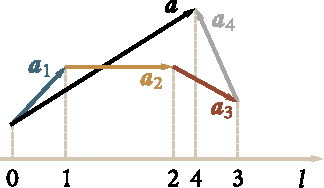
\includegraphics[scale=1]{figures/ch_01/fig_1_11.pdf}
			\caption[]{}
			\label{fig:1_11}
		\end{center}
	\end{minipage}
	\hfill{ }%\hspace{-0.1cm}
	\begin{minipage}[t]{0.5\linewidth}
		\begin{center}
			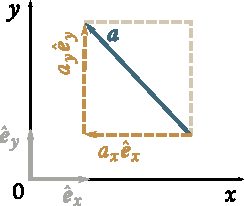
\includegraphics[scale=0.95]{figures/ch_01/fig_1_12.pdf}
			\caption[]{}
			\label{fig:1_12}
		\end{center}
	\end{minipage}
	\vspace{-0.8cm}
\end{figure}

Inspection of \fig{1_12} shows that the vector $\vec{a}$ can be represented in the form of a linear combination of the unit vectors $\vecuni{x}$ and $\vecuni{y}$ [see \eqn{1_5}]:
\begin{equation*}
\vec{a} = a_x \vecuni{x} + a_y \vecuni{y}.
\end{equation*}

\noindent
The projections of the vector onto the coordinate axes play the part of the coefficients $\alpha$ and $\beta$. In the example being considered, the projection $a_x$ is negative, therefore the vector $a_x\vecuni{x}$ has a direction opposite to that of the unit vector $\vecuni{x}$.

We took the vector $\vec{a}$ perpendicular to the $z$-axis owing to which $a_z=0$. In the general case when all three projections of a vector differ from zero, we have
\begin{equation}\label{eq:1_9}
\vec{a} = a_x \vecuni{x} + a_y \vecuni{y} + a_z \vecuni{z},
\end{equation}

\noindent
Thus, any vector can be expressed through its projections onto the coordinate axes and the unit vectors of these axes. Therefore, the projections of a vector onto the coordinate axes are called its \textbf{components}.

The components $a_x$, $a_y$, $a_z$ equal (with an accuracy to the sign) the sides of a right parallelepiped in which the vector $\vec{a}$ is the major diagonal (\fig{1_13}). We therefore have
\begin{equation}\label{eq:1_10}
a^2 = a_x^2 + a_y^2 + a_z^2.
\end{equation}

Assume that $\vec{c}=\vec{a}+\vec{b}$. Representing each of these vectors in accordance with \eqn{1_9}, we get
\begin{equation*}
c_x\vecuni{x} + c_y\vecuni{y} + a_z\vecuni{z} = (a_x+b_x)\vecuni{x} + (a_y+b_y)\vecuni{y} + (a_z+b_z)\vecuni{z}
\end{equation*}

\noindent
(we have factored out $\vecuni{x}$, $\vecuni{y}$, and $\vecuni{z}$)· Equal vectors have identical projections onto the coordinate axes. On these grounds, we can write that
\begin{equation}\label{eq:1_11}
c_x=a_x+b_x,\quad c_y=a_y+b_y,\quad a_z=a_z+b_z
\end{equation}

\noindent
[compare with \eqn{1_8}]. Equations~\eqref{eq:1_11} express analytically the rule of vector addition. They hold for any number of addends.

\textbf{Position Vector.} The position vector (or radius vector) $\vec{r}$ of a point is defined as the vector drawn from the origin of coordinates to the given point (\fig{1_14}). Its projections onto the coordinate axes equal the Cartesian coordinates of the given point:
\begin{equation}\label{eq:1_12}
r_x=x,\quad r_y=y,\quad r_z=z.
\end{equation}

\noindent
Consequently, in accordance with \eqn{1_9}, the position vector can be represented in the form
\begin{equation}\label{eq:1_13}
\vec{r} = x\vecuni{x} + y\vecuni{y} + z\vecuni{z}.
\end{equation}

\noindent
By \eqn{1_10}, we have
\begin{equation}\label{eq:1_14}
r^2 = x^2 + y^2 + z^2.
\end{equation}

\begin{figure}[t]
	\begin{minipage}[t]{0.5\linewidth}
		\begin{center}
			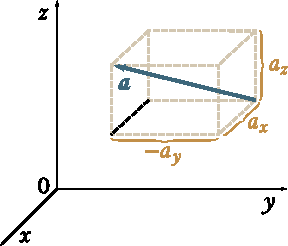
\includegraphics[scale=1]{figures/ch_01/fig_1_13.pdf}
			\caption[]{}
			\label{fig:1_13}
		\end{center}
	\end{minipage}
	\hfill{ }%\hspace{-0.1cm}
	\begin{minipage}[t]{0.5\linewidth}
		\begin{center}
			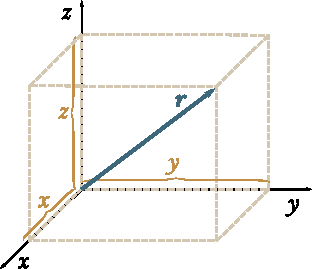
\includegraphics[scale=0.95]{figures/ch_01/fig_1_14.pdf}
			\caption[]{}
			\label{fig:1_14}
		\end{center}
	\end{minipage}
\vspace{-0.3cm}
\end{figure}

\begin{figure}[t]
	\begin{center}
		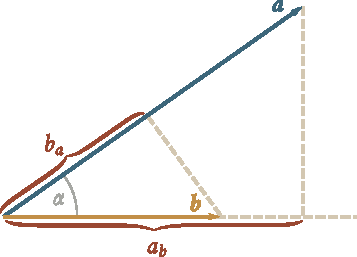
\includegraphics[scale=0.9]{figures/ch_01/fig_1_15.pdf}
		\caption[]{}
		\label{fig:1_15}
	\end{center}
	\vspace{-1.0cm}
\end{figure}

\textbf{The Scalar Product of Vectors.} Two vectors $\vec{a}$ and $\vec{b}$ can be multiplied by each other in two ways. One of them results in a scalar quantity, and the other in a certain new vector. Accordingly, two products of vectors are distinguished---the scalar product and the vector product. It must be noted that \textit{the operation of dividing a vector by a vector does not exist}.

The scalar product of the vectors $\vec{a}$ and $\vec{b}$ is defined as the scalar quantity equal to the product of the magnitudes of these vectors and the cosine of the angle $\alpha$ between them:
\begin{equation}\label{eq:1_15}
\vecdot{a}{b} = ab\sin\alpha
\end{equation}

\noindent
(\fig{1_15}). When writing a scalar product, the symbols of the vectors being multiplied are usually written next to each other with dot between them (this is why a scalar product is also called a dot product; sometimes nothing is used between the symbols)\footnote{The dot symbol between vectors is preferred in the \LaTeX version to adopt a more modern approach.}. Equation~\eqref{eq:1_15} expresses an algebraic quantity: when $\alpha$ is acute, we have $\vecdot{a}{b}>0$, and when it is obtuse, we have $\vecdot{a}{b}<0$. The scalar product of mutually perpendicular vectors ($\alpha=\pi/2$) equals zero.

It must be noted that by the square of a vector is always meant the scalar product of this vector by itself:
\begin{equation}\label{eq:1_16}
\vec{a}^2 = \vecdot{a}{a} = aa\cos\alpha = a^2.
\end{equation}

\noindent
Thus, the square of a vector equals the square of its magnitude. In particular, the square of any unit vector equals unity:
\begin{equation}\label{eq:1_17}
\vecuni{x}^2 = \vecuni{y}^2 = \vecuni{z}^2 = 1.
\end{equation}

\noindent
We shall note in passing that owing to the unit vectors being mutually perpendicular, scalar products such as $\vecunidot{i}{k}$, equal zero if $i\neq k$.

The Kronecker symbol or delta $\delta_{ik}$ is very convenient. It is determined as follows:
\begin{equation}\label{eq:1_18}
\delta_{ik} = \begin{cases}
1, &\mbox{if } i = k, \\
0, &\mbox{if } i\neq k. \end{cases}
\end{equation}

\noindent
When this symbol is used, the properties of the scalar products of the coordinate axis unit vectors established above can be expressed by a single formula:
\begin{equation}\label{eq:1_19}
\vecunidot{i}{k} = \delta_{ik}\quad (i, k = x, y, z)
\end{equation}

\noindent
where the subscripts $i$ and $k$ can assume any of the values $x$, $y$ and $z$ independently of each other.

It follows from the definition~\eqref{eq:1_15} that a scalar product is commutative, \ie, it does not depend on the sequence of the multipliers:
\begin{equation}\label{eq:1_20}
\vecdot{a}{b} = \vecdot{b}{a}.
\end{equation}

\noindent
Equation~\eqref{eq:1_15} can be written in several ways:
\begin{equation*}
\vecdot{a}{b} = ab\cos\alpha = (a\cos\alpha)\,b = a\,(b\cos\alpha).
\end{equation*}

\noindent
Examination of \fig{1_15} shows that $a\cos\alpha$ equals $a_b$---the projection of the vector $\vec{a}$ onto the direction of the vector $\vec{b}$. Similarly, $b\cos\alpha= b_a$---the projection of the vector $\vec{b}$ onto the direction of the vector $\vec{a}$. We can therefore say that the scalar product of two vectors is defined as the scalar quantity equal to the product of the magnitude of one of the vectors being multiplied and the projection of the second vector onto the direction of the first one:
\begin{equation}\label{eq:1_21}
\vecdot{a}{b} = a_b b = a b_a.
\end{equation}

Taking into account that the projection of the sum of vectors equals the sum of the projections of the vectors being added, we can write that
\begin{equation}\label{eq:1_22}
\vec{a}\boldsymbol{\cdot}(\vec{b}+\vec{c}+\ldots) = a(\vec{b}+\vec{c}+\ldots)_a = a(b_a+c_a+\ldots) = ab_a+ac_a+\ldots = ab+ac+\ldots .
\end{equation}

\noindent
Hence, it follows that the scalar product of vectors is distributive---the product of the vector $\vec{a}$ and the sum of several vectors equals the sum of the products of the vector $\vec{a}$ and each of the added vectors taken separately.

Let us represent the vectors being multiplied in the form of \eqn{1_9} and take advantage of the distributive nature of a scalar product. We get
\begin{align*}
\vecdot{a}{b} &= (a_x\vecuni{x} + a_y\vecuni{y} + a_z\vecuni{z})(b_x\vecuni{x} + b_y\vecuni{y} + b_z\vecuni{z})\\
&= a_xb_x\vecunidot{x}{x} + a_xb_y\vecunidot{x}{y} + a_xb_z\vecunidot{x}{z} + a_yb_x\vecunidot{y}{x} + a_yb_y\vecunidot{y}{y}\\
&\,+ a_yb_z\vecunidot{y}{z}+ a_zb_x\vecunidot{z}{x} + a_zb_y\vecunidot{z}{y} + a_zb_z\vecunidot{z}{z}.
\end{align*}

\noindent
Now let us take \eqn{1_19} into consideration. As a result, we get an expression for a scalar product through the projections of the vectors being multiplied:
\begin{equation}\label{eq:1_23}
\vecdot{a}{b} = a_xb_x + a_yb_x + a_zb_z.
\end{equation}

\noindent
It must be noted that when the coordinate axes are rotated, the projections of vectors onto these axes change. The quantity $ab\cos\alpha$ does not depend on the choice of the axes, however. We thus conclude that the changes in the projections of the vectors $\vec{a}$ and $\vec{b}$, when the axes are rotated, are of a nature such that their combination of the form of \eqn{1_23} remains invariant (unchanged):
\begin{equation}\label{eq:1_24}
\vecdot{a}{b} = a_xb_x + a_yb_x + a_zb_z = \mathrm{inv}.
\end{equation}

It is a simple matter to see that the projection of the vector $\vec{a}$ onto the direction $l$ [see \eqn{1_7}] can be represented in the form
\begin{equation}\label{eq:1_25}
a_l = \vec{a}\boldsymbol{\cdot}\vecuni{l},
\end{equation}

\noindent
where $\vecuni{l}$ is the unit vector of the direction $l$. Similarly,
\begin{equation}\label{eq:1_26}
a_x = \vec{a}\boldsymbol{\cdot}\vecuni{x},\quad  a_y = \vec{a}\boldsymbol{\cdot}\vecuni{y}, \quad  a_z=\vec{a}\boldsymbol{\cdot}\vecuni{z}.
\end{equation}

\textbf{The Vector Product.} The vector product of the vectors $\vec{a}$ and $\vec{b}$ is defined as the vector $\vec{c}$ determined by the equation
\begin{equation}\label{eq:1_27}
\vec{c} = ab\sin(\alpha)\hatvec{n},
\end{equation}

\noindent
where $a$ y $b$ magnitudes of the vectors being multiplied, $\alpha$, is the angle between the vectors, $\hatvec{n}$, is the unit vector of a normal\footnote{The symbol $\hatvec{n}$ is simpler and more illustrative than $\vecuni{n}$.} to the plane containing the vectors $\vec{a}$ and $\vec{b}$ (\fig{1_16}).

The direction of $\hatvec{n}$ is chosen so that the sequence of the vectors $\vec{a}$, $\vec{b}$, $\hatvec{n}$ forms a right-handed system. This signifies that if we look along the vector $\hatvec{n}$, then the shortest path in rotation from the first multiplier to the second one will be clockwise. In \fig{1_16}, the vector $\hatvec{n}$ is directed beyond the drawing, and it is therefore depicted by a circle with a cross\footnote{We shall depict vectors perpendicular to the plane of a drawing by a circle with a cross in it if the vector is directed away from us, and by a circle with a point at its centre if the vector is directed toward us. For clarity, we can imagine a vector in the form of an arrow with a tapered tip and cross-shaped feathers on its tail. Thus, when the vector is directed toward us (the arrow is flying toward us), we see a circle with a point; when the vector is directed away from us (the arrow is flying away from us), we see a circle with a cross.}. The direction of the vector $\vec{c}$ coincides with that of $\hatvec{n}$.

%\begin{figure}[t]
%	\begin{center}
%		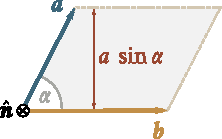
\includegraphics[scale=1]{figures/ch_01/fig_1_16.pdf}
%		\caption[]{}
%		\label{fig:1_16}
%	\end{center}
%	\vspace{-0.7cm}
%\end{figure}

A vector product is usually designated in one of two ways:
\begin{equation*}
[\vec{a},\vec{b}]\quad\text{or }\quad \vec{a}\times\vec{b}
\end{equation*}

\noindent
the latter notation resulting in the term cross product sometimes being used to signify a vector product. We shall use the latter notation\footnote{To avoid confusion, in the \LaTeX version, we shall use the cross product symbol.}. Thus, according to \eqn{1_27}, we have
\begin{equation}\label{eq:1_28}
\vecprod{a}{b} = (ab\sin\alpha)\hatvec{n}.
\end{equation}

A glance at \fig{1_16} shows that the magnitude of a vector product has a simple geometrical meaning---the expression $ab\sin\alpha$ numerically equals the area of a parallelogram constructed on the vectors being multiplied.

We determined the direction of the vector $\vecprod{a}{b}$ by relating it to the direction of rotation from the first multiplier to the second one. When considering vectors such as the position vector $\vec{r}$, the velocity $\vec{v}$, and the force $\vec{F}$, the choice of their direction is quite obvious---it follows from the nature of these quantities themselves. Such vectors are called \textbf{polar} or \textbf{true}. Vectors of the type $\vecprod{a}{b}$ whose direction is related to that of rotation are called axial or \textbf{pseudovectors}. When conditions change, for example, upon going over from a right-hand system of coordinates to a left-hand one, the directions of pseudovectors are reversed, while those of true vectors remain unchanged.

It must be borne in mind that a vector product will be a pseudovector only when both of the vectors being multiplied are true (or both are pseudovectors). The vector product of a true vector and a pseudovector will be true. Reversing of a condition determining the direction of a pseudovector will lead in this case to a change in the sign in front of the vector product and also to a change in the sign of one of the multipliers. As a result, the quantity expressed
by the vector product remains unchanged.

Since the direction of a vector product is determined by the direction of rotation from the first multiplier to the second one, the result of vector multiplication depends on the order of the multipliers. Transposition of the multipliers leads to reversing of the direction of the resultant vector. Thus, a vector product does not have the property of commutativity:
\begin{equation}\label{eq:1_29}
\vecprod{a}{b} = -\vecprod{b}{a}.
\end{equation}

\noindent
A vector product can be proved to be distributive, \ie, it can be shown that
\begin{equation}\label{eq:1_30}
\vec{a}\times(\vec{b}_1+\vec{b}_2+\ldots)] = \vec{a}\times\vec{b}_1 + \vec{a}\times\vec{b}_2 + \ldots.
\end{equation}

%\begin{figure}[t]
%	\begin{center}
%		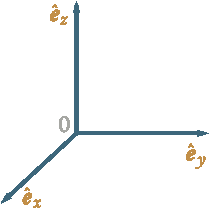
\includegraphics[scale=1]{figures/ch_01/fig_1_17.pdf}
%		\caption[]{}
%		\label{fig:1_17}
%	\end{center}
%	\vspace{-1.0cm}
%\end{figure}
\begin{figure}[t]
	\begin{minipage}[t]{0.5\linewidth}
		\begin{center}
			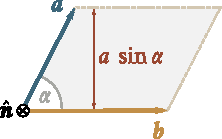
\includegraphics[scale=1]{figures/ch_01/fig_1_16.pdf}
			\caption[]{}
			\label{fig:1_16}
		\end{center}
	\end{minipage}
	\hfill{ }%\hspace{-0.1cm}
	\begin{minipage}[t]{0.5\linewidth}
		\begin{center}
			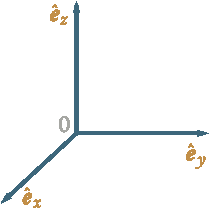
\includegraphics[scale=1]{figures/ch_01/fig_1_17.pdf}
			\caption[]{}
			\label{fig:1_17}
		\end{center}
	\end{minipage}
	\vspace{-0.3cm}
\end{figure}

Let us consider the vector products of the unit vectors of the coordinate axes (\fig{1_17}). In accordance with the definition~\eqref{eq:1_28}, we have
\begin{align}
\vecuniprod{x}{x} &= \vecuniprod{y}{y} = \vecuniprod{z}{z} = 0,\nonumber\\
\vecuniprod{x}{y} &= -\vecuniprod{y}{x} = \vecuni{z},\label{eq:1_31}\\
\vecuniprod{y}{z} &= -\vecuniprod{z}{y} = \vecuni{x},\nonumber\\
\vecuniprod{z}{x} &= -\vecuniprod{x}{z} = \vecuni{y}.\nonumber
\end{align}

\noindent
Representing the vectors being multiplied in the form of \eqn{1_9} and taking advantage of the distributivity of a vector product, we get:
\begin{align*}
\vecprod{a}{b} &= (a_x\vecuni{x}+a_y\vecuni{y}+a_z\vecuni{z})\times(b_x\vecuni{x}+b_y\vecuni{y}+b_z\vecuni{z})\\
&= a_xb_x\vecuniprod{x}{x} + a_xb_y\vecuniprod{x}{y} + a_xb_z\vecuniprod{x}{z}\\
&+ a_yb_x\vecuniprod{y}{x} + a_yb_y\vecuniprod{y}{y} + a_yb_z\vecuniprod{y}{z}\\
&+ a_zb_x\vecuniprod{z}{x} + a_zb_y\vecuniprod{z}{y} + a_zb_z\vecuniprod{z}{z}
\end{align*}

\noindent
Taking into account relation~\eqref{eq:1_31}, we arrive at the following expression:
\begin{equation}\label{eq:1_32}
\vecprod{a}{b} = \vecuni{x}(a_yb_z - a_zb_y) + \vecuni{y}(a_zb_x - a_xb_z) + \vecuni{z}(a_xb_y - a_yb_x).
\end{equation}

\noindent
The above expression can be represented in the form of a determinant
\begin{equation}\label{eq:1_33}
\vecprod{a}{b} = \begin{vmatrix}
\vecuni{x} & \vecuni{y} & \vecuni{z}\\
a_x & a_y & a_z\\
b_x & b_y & b_z
\end{vmatrix}.
\end{equation}

\begin{figure}[t]
	\begin{center}
		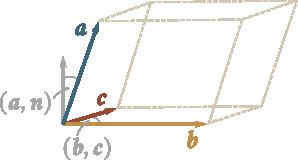
\includegraphics[scale=1]{figures/ch_01/fig_1_18.pdf}
		\caption[]{}
		\label{fig:1_18}
	\end{center}
	\vspace{-0.7cm}
\end{figure}

\textbf{Scalar Triple Product.} A scalar triple product of three vectors is defined as the expression $\vecmix{a}{b}{c}$, \ie, the scalar product of the vector $\vec{a}$ and the vector product of the vectors $\vec{b}$ and $\vec{c}$. According to the definitions~\eqref{eq:1_15} and~\eqref{eq:1_28}, we have
\begin{equation*}
\vecmix{a}{b}{c} = a\{bc\sin(\vec{b}, \vec{c})\}\cos(\vec{a},\hatvec{n}).
\end{equation*}

\noindent
Here $(\vec{b},\vec{c})$ is the angle between $\vec{b}$ and $\vec{c}$, and $(\vec{a},\hatvec{n})$ is the angle between the vector $\vec{a}$ and the unit vector $\hatvec{n}$ determining the direction of the vector $\vecprod{b}{c}$. Inspection of \fig{1_18} shows that the expression $bc\sin(\vec{b},\vec{c})$ numerically equals the area of the base of a parallelepiped constructed on the vector being multiplied, while the expression $a\cos(\vec{a},\hatvec{n})$ numerically equals the altitude of this parallelepiped taken with the plus sign if the angle $(\vec{a},\hatvec{n})$ is acute, and with the minus sign if it is obtuse. Consequently, the expression $\vecmix{a}{b}{c}$ has a simple geometrical meaning---it numerically equals the volume of a parallelepiped constructed on the vectors being multiplied [taken with the plus or minus sign depending on the value of the angle $(\vec{a},\hatvec{n})$]. In calculating the volume of a parallelepiped, the result cannot depend on which of its faces is taken as the base. Hence, it follows that
\begin{equation}\label{eq:1_34}
\vecmix{a}{b}{c} = \vecmix{b}{c}{a} = \vecmix{c}{a}{b}.
\end{equation}

\noindent
Thus, a scalar triple product permits cyclic transposition of the multipliers, \ie, substitution for each of the multipliers of the one following it in the cycle:
\begin{equation*}
% \begin{tikzcd}
% \vec{a}\arrow[rd] &\\
% \vec{c}\arrow[u] & \arrow[l] \vec{b}
% \end{tikzcd}
\begin{tikzcd}[column sep=small]
             & \vec{a} \arrow[rd] &              \\
\vec{c} \arrow[ru] &              & \vec{b} \arrow[ll]
\end{tikzcd}
\end{equation*}

\textbf{Vector Triple Product.} Let us consider a vector triple product of the three vectors $\vec{a}$, $\vec{b}$ and $\vec{c}$
\begin{equation*}
\vec{d} = \vec{a}\times\vecprod{b}{c}.
\end{equation*}

\noindent
Any vector product is perpendicular to both multipliers. Therefore, the vector $\vec{d}$ is perpendicular to the unit vector $\hatvec{n}$ determining the direction of the vector $\vecprod{b}{c}$. Hence, it follows that the vector $\vec{d}$ is in the plane formed by the vectors $\vec{b}$ and $\vec{c}$ and, consequently, can be represented as a linear combination of these vectors:
\begin{equation*}
\vec{d} = \alpha\vec{b} + \beta\vec{c}
\end{equation*}

\noindent
[see \eqn{1_5}]. We find from the relevant calculations that $\alpha=\vecdot{a}{c}$ and $\beta=-\vecdot{a}{b}$. Thus,
\begin{equation}\label{eq:1_35}
\vec{a}\times\vecprod{b}{c} = \vec{b}(\vecdot{a}{c}) - \vec{c}(\vecdot{a}{b}).
\end{equation}

\textbf{Derivative of a Vector.} Let us consider a vector that changes in time according to a known law $\vec{a}(t)$. The projections of this vector onto the coordinate axes are preset functions of time. Hence,
\begin{equation}\label{eq:1_36}
\vec{a}(t) = \vecuni{x}a_x(t) + \vecuni{y}a_y(t) + \vecuni{z}a_z(t)
\end{equation}

\noindent
(we assume that the coordinate axes do not rotate in space so that their unit vectors do not change with time).

Let the vector projections receive the increments $\Delta a_x$, $\Delta a_y$, $\Delta a_z$ during the time $\Delta t$. The vector therefore receives the increment $\Delta\vec{a} = \vecuni{x}\Delta a_x + \vecuni{y}\Delta a_y + \vecuni{z}\Delta a_z$. The rate of change of the vector $\vec{a}$ with time can be characterized by the ratio of $\Delta\vec{a}$ to $\Delta t$:
\begin{equation}\label{eq:1_37}
\frac{\Delta\vec{a}}{\Delta t} = \vecuni{x}\frac{\Delta a_x}{\Delta t} + \vecuni{y}\frac{\Delta a_y}{\Delta t} + \vecuni{z}\frac{\Delta a_z}{\Delta t}.
\end{equation}

\noindent
This expression gives the mean rate of change of $\vec{a}$ during the time interval $\Delta t$. Let us assume that $\vec{a}$ changes continuously with time, without any jumps. Consequently, the smaller the interval $\Delta t$, the more accurately does the value of \eqn{1_37} characterize the rate of change in $\vec{a}$ at the moment $t$ preceding the interval $\Delta t$. Therefore, the rate of change in the vector $\vec{a}$ at the moment $t$ equals the limit of \eqn{1_37} obtained when $\Delta t$ tends to zero:
\begin{align}
\text{the rate of change in }\vec{a} &= \lim_{\Delta t\to 0}\frac{\Delta\vec{a}}{\Delta t} \nonumber\\
&= \vecuni{x} \lim_{\Delta t\to 0}\frac{\Delta a_x}{\Delta t} + \lim_{\Delta t\to 0}\vecuni{y} \frac{\Delta a_y}{\Delta t} + \lim_{\Delta t\to 0}\vecuni{z} \frac{\Delta a_z}{\Delta t}.\label{eq:1_38}
\end{align}

If there is a function $f(t)$ of the argument $t$, then the limit of the ratio of the increment of the function $\Delta f$ to the increment of the argument $\Delta t$ obtained when $\Delta t$ tends to zero is called the derivative of the function $f$ with respect to $t$ and is designated by the symbol $\diffin{f}{t}$. Expression~\eqref{eq:1_38} can therefore be written as follows:
\begin{equation}\label{eq:1_39}
\diff{\vec{a}}{t} = \vecuni{x}\diff{a_x}{t} + \vecuni{y}\diff{a_y}{t} + \vecuni{z}\diff{a_z}{t}.
\end{equation}

\noindent
The result obtained signifies that the projections of the vector $\diffin{\vec{a}}{t}$ onto the coordinate axes equal the time derivatives of the projections of the vector $\vec{a}$:
\begin{equation}\label{eq:1_40}
\left(\diff{\vec{a}}{t}\right)_{\text{pr. }x} = \diff{a_x}{t},\quad \left(\diff{\vec{a}}{t}\right)_{\text{pr. }y} = \diff{a_y}{t},\quad \left(\diff{\vec{a}}{t}\right)_{\text{pr. }z} = \diff{a_z}{t},\quad.
\end{equation}

It is customary practice in physics to denote time derivatives by the symbol of the corresponding quantity with a dot over it, for example,
\begin{equation}\label{eq:1_41}
\diff{\varphi}{t} = \dot{\varphi},\quad \diffsec{\varphi}{t} = \ddot{\varphi},\quad \diff{\vec{a}}{t} = \dot{\vec{a}},\quad \diffsec{\vec{a}}{t} = \ddot{\vec{a}}.
\end{equation}

\noindent
Using this notation, we can write equation~\eqref{eq:1_39} as follows:
\begin{equation}\label{eq:1_42}
\dot{\vec{a}} = \vecuni{x}\dot{a}_x + \vecuni{y}\dot{a}_y + \vecuni{z}\dot{a}_z.
\end{equation}

\noindent
If we take the position vector $\vec{r}(t)$ of a moving point as $\vec{a}(t)$, then by \eqn{1_42} we have
\begin{equation}\label{eq:1_43}
\dot{\vec{r}} = \vecuni{x}\dot{r}_x + \vecuni{y}\dot{r}_y + \vecuni{z}\dot{r}_z,
\end{equation}

\noindent
where $x$, $y$, $z$ are functions of $t$, namely, $x=x(t)$, $y=t(t)$, $z=z(t)$.

The differential (``increment'') of the function $f(t)$ is defined as the expression
\begin{equation}\label{eq:1_44}
\mathrm{d}f = f'\, \mathrm{d}t,
\end{equation}

\noindent
where $f'$ is the derivative of $f$ with respect to $t$.  According to \eqn{1_39}, the differential of the vector $\vec{a}$ is determined by the equation
\begin{equation}\label{eq:1_45}
\mathrm{d}\vec{a} = \vecuni{x}\mathrm{d}a_x + \vecuni{y}\mathrm{d}a_y + \vecuni{z}\mathrm{d}a_z.
\end{equation}

In particular,
\begin{equation}\label{eq:1_46}
\mathrm{d}\vec{r} = \vecuni{x}\mathrm{d}x + \vecuni{y}\mathrm{d}y + \vecuni{z}\mathrm{d}z.
\end{equation}

It must be noted that the increment of a function during a very short, but finite interval $\Delta t$ approximately equals
\begin{equation}\label{eq:1_47}
\Delta f \approx f'\Delta t = \diff{f}{t}\Delta t.
\end{equation}

\noindent
In the limit, when $\Delta t\to 0$, the approximate equation~\eqref{eq:1_47} transforms into the accurate equation~\eqref{eq:1_44}.

A similar equation to~\eqref{eq:1_47} can also be written for the vector function
\begin{equation}\label{eq:1_48}
\Delta\vec{a} \approx \diff{\vec{a}}{t}\Delta t.
\end{equation}

\textbf{Derivative of the Product of Functions.} We shall consider the function $\vec{b}(t)$ that equals the product of the scalar function $\varphi(t)$ and the vector function $\vec{a}(t)$, \ie, $\vec{b}(t)=\varphi(t)\vec{a}(t)$ or, more briefly, $\vec{b}=\varphi\vec{a}$. Let us find the increment of the function $\vec{b}$:
\begin{equation*}
\Delta\vec{b} = \Delta(\varphi\vec{a}) = (\varphi + \Delta\varphi)(\vec{a} + \Delta\vec{a}) - \varphi\vec{a} = \varphi\Delta\vec{a} + \vec{a}\Delta\varphi + \Delta\varphi\Delta\vec{a}.
\end{equation*}

\noindent
Representing the increments of the functions in the form of expressions~\eqref{eq:1_47} and \eqref{eq:1_48}, we get:
\begin{equation*}
\Delta\vec{b} \approx \varphi\diff{\vec{a}}{t}\Delta t + \vec{a}\diff{\varphi}{t}\Delta t + \diff{\varphi}{t}\diff{\vec{a}}{t}(\Delta t)^2
\end{equation*}

\noindent
whence
\begin{equation*}
\frac{\Delta\vec{b}}{\Delta t} \approx \varphi\diff{\vec{a}}{t} + \vec{a}\diff{\varphi}{t} + \diff{\varphi}{t}\diff{\vec{a}}{t}\Delta t.
\end{equation*}

\noindent
In the limit when $\mathrm{d}t$ tends to zero, this approximate equation transforms into an accurate one. Thus,
\begin{equation*}
\diff{\vec{b}}{t} = \lim_{\Delta t\to 0} \diff{\vec{b}}{t} =  \lim_{\Delta t\to 0} \left(\varphi\diff{\vec{a}}{t} + \vec{a}\diff{\varphi}{t} + \diff{\varphi}{t} \diff{\vec{a}}{t}\Delta t\right).
\end{equation*}

\noindent
The first two addends do not depend on $\Delta t$ and therefore do not change when going over to the limit. The limit of the third addend equals zero. Hence, substituting $\varphi\vec{a}$ for $\vec{b}$, we obtain
\begin{equation}\label{eq:1_49}
\diff{(\varphi\vec{a})}{t} = \varphi\diff{\vec{a}}{t} + \vec{a}\diff{\varphi}{t} = \varphi\dot{\vec{a}}+\dot{\varphi}\vec{a}.
\end{equation}

Now let us consider the scalar product of two vector functions $\vec{a}(t)$ and $\vec{b}(t)$. The increment of this product is
\begin{align*}
\Delta(\vec{a}\vec{b}) &= (\vec{a} + \Delta\vec{a})(\vec{b} + \Delta\vec{b}) - \vec{a}\vec{b}\\
&= \vec{a}\Delta\vec{b} + \vec{b}\Delta\vec{a} + \Delta\vec{a}\Delta\vec{b} \\
&\approx \vec{a}\dot{\vec{b}}\Delta t + \vec{b}\dot{\vec{a}}\Delta t + \dot{\vec{a}}\dot{\vec{b}}(\Delta t)^2
\end{align*}

\noindent
Hence
\begin{equation*}
\diff{(\vec{a}\vec{b})}{t} = \lim_{\Delta t\to 0} \frac{\Delta(\vec{a}\vec{b})}{\Delta t} = \lim_{\Delta t\to 0} (\vec{a}\dot{\vec{b}} + \vec{b}\dot{\vec{a}} + \dot{\vec{a}}\dot{\vec{b}}\Delta t)
\end{equation*}

\noindent
or finally
\begin{equation}\label{eq:1_50}
\diff{(\vec{a}\vec{b})}{t} = \vec{a}\dot{\vec{b}} + \vec{b}\dot{\vec{a}}.
\end{equation}

\noindent
Multiplying \eqn{1_50} by $\mathrm{d}t$, we get a differential:
\begin{equation}\label{eq:1_51}
\diff{(\vec{a}\vec{b})}{t} = \vec{a}\dot{\vec{b}} + \vec{b}\dot{\vec{a}}.
\end{equation}

Let us calculate the derivative and the differential of the square of a vector function. According to Eqs.~\eqref{eq:1_50} and~\eqref{eq:1_51}, we have
\begin{align}
\diff{\vec{a}^2}{t} &= 2\vec{a}\dot{\vec{a}},\label{eq:1_52}\\
\mathrm{d}(\vec{a}^2) &= 2\vec{a}\,\mathrm{d}\vec{a},\label{eq:1_53}
\end{align}

\noindent
Taking into account that $\vec{a}^2 = a^2$ [see \eqn{1_16}], we can write:
\begin{equation}\label{eq:1_54}
2\vec{a}\,\mathrm{d}\vec{a} = \mathrm{d}(a^2) \quad \text{or} \quad \vec{a}\,\mathrm{d}\vec{a} = \mathrm{d}\left(\frac{a^2}{2}\right).
\end{equation}

Finally, let us consider the derivative of the vector product of the functions $\vec{a}(t)$ and $\vec{b}(t)$. The increment of the function being considered is
\begin{align*}
\Delta\vecprod{a}{b} &= [(\vec{a} + \Delta\vec{a}),(\vec{b} + \Delta\vec{b}) - \vecprod{a}{b}]\\
&= [\vec{a},\Delta\vec{b}] + [\Delta\vec{a},\vec{b}] + [\Delta\vec{a},\Delta\vec{b}]\\
&\approx [\vec{a},\dot{\vec{b}}\Delta t] + [\dot{\vec{a}}\Delta t,\vec{b}] + [\dot{\vec{a}}\Delta t,\dot{\vec{b}}\Delta t].
\end{align*}

\noindent
Correspondingly,
\begin{equation*}
\frac{\upd}{\deriv{t}}(\vecprod{a}{b}) = \lim_{\Delta t\to 0} \{[\vec{a},\dot{\vec{b}}] + [\dot{\vec{a}},\vec{b}] + [\dot{\vec{a}},\dot{\vec{b}}]\Delta t\}.
\end{equation*}

\noindent
After a limit transition, we arrive at the equation
\begin{equation}\label{eq:1_55}
\frac{\upd}{\deriv{t}}(\vecprod{a}{b}) = [\vec{a},\dot{\vec{b}}] + [\dot{\vec{a}},\vec{b}].
\end{equation}

\textbf{Derivative of a Unit Vector.} Let us consider the unit vector $\vecuni{a}$ of the vector $\vec{a}$. It is obvious that the vector $\vecuni{a}$ can change only in direction. Assume that during the very short interval $\Delta t$ the vector $\vec{a}$ and together with it the unit vector $\vecuni{a}$ rotate through the angle $\Delta\varphi$ (\fig{1_19}). At a low value of $\Delta\varphi$, the magnitude of the vector $\Delta\vecuni{a}$ approximately equals the angle $\Delta\varphi$, namely, $|\Delta\vecuni{a}|\approx\Delta\varphi$ (the segment depicting $\Delta\vecuni{a}$ is the base of an isosceles triangle with sides equal to unity). We must note that the smaller is $\Delta\varphi$, the more accurate is our approximate equation. The vector $\Delta\varphi$ itself can be represented in the form
\begin{equation*}
\Delta\vecuni{a} = |\Delta\vecuni{a}| \boldsymbol{\cdot} \vecuni{\Delta\vec{e}} \approx \Delta\varphi \boldsymbol{\cdot} \vecuni{\Delta\vec{e}}
\end{equation*}

\noindent
where $\vecuni{\Delta\vec{e}}$ is the unit vector of the vector $\Delta\vecuni{a}$. When $\Delta\varphi$ tends to zero, the unit vector $\vecuni{\Delta\vec{e}}$ will rotate and in the limit coincide with the unit vector $\vecuni{\perp}$ perpendicular to $\vecuni{a}$ (see \fig{1_19}).

The derivative of $\vecuni{a}$ with respect to $t$, by definition, is
\begin{equation*}
\diff{\vecuni{a}}{t} = \lim_{\Delta t\to 0} \frac{\Delta\vecuni{a}}{\Delta t} = \lim_{\Delta t\to 0} \frac{\Delta\varphi}{\Delta t}\vecuni{\Delta\vec{e}} = \diff{\varphi}{t}\vecuni{\perp}.
\end{equation*}

\noindent
Thus,
\begin{equation}\label{eq:1_56}
\dot{\hat{\vec{e}}}_{a} = \dot{\varphi}\vecuni{\perp}.
\end{equation}

\noindent
The quantity $\dot{\varphi}=\diffin{\varphi}{t}$ is the angular velocity of rotation of the vector $\vec{a}$ (see Sec.~\ref{sec:1_5}). The unit vector $\vecuni{\perp}$ is in the plane in which the vector $\vec{a}$ is rotating at the given moment, and its sense is in the direction of rotation.

\begin{figure}[t]
	\begin{center}
		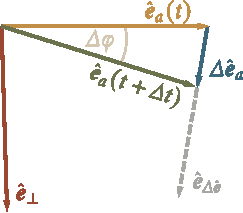
\includegraphics[scale=0.95]{figures/ch_01/fig_1_19.pdf}
		\caption[]{}
		\label{fig:1_19}
	\end{center}
	\vspace{-0.7cm}
\end{figure}

\section{Velocity and Speed}\label{sec:1_3}

A point particle in motion travels along a certain line. The latter is called its path or trajectory\footnote{It must be noted that the concept of a trajectory can be applied only to a ``classical'' particle to which accurate values of its coordinate and momentum (\ie, velocity) can be ascribed at each moment of time. According to quantum mechanics, real particles can be characterized with the aid of a coordinate and momentum only with a certain accuracy. The limit of this accuracy is determined by the equation of Heisenberg's uncertainty principle: $\Delta x\Delta p\gtrsim\hbar$. Here $\Delta x$ is the uncertainty in the coordinate of a particle, $\Delta p$ is the uncertainty in its momentum, and $\hbar$ is Planck's constant $h$ divided by $2\pi$, \ie, $\hbar = h/2\pi = \SI{1.05e-34}{\joule\second}$. The sign $\gtrsim$ signifies ``greater than a value of the order of''. Replacing the momentum with the product of the mass and the velocity, we can write $\Delta x\Delta v\gtrsim\hbar/m$. It can be seen from this relation that the smaller the mass of a particle, the more uncertain do its coordinate and velocity become, and, consequently, the less applicable is the concept of trajectory. For macroscopic bodies (\ie, bodies formed by a very great number of molecules), the uncertainties in the coordinate and velocity do not exceed the practically attainable accuracy of measuring these quantities. Hence, the concept of trajectory may be applied to such bodies without any reservations. For microparticles (electrons, protons, neutrons, separate atoms and molecules), the concept of trajectory either cannot be applied at all, or can be applied with a limited accuracy, depending on the conditions in which motion occurs. For example, the motion o electrons in a cathode-ray tube can approximately be considered as occurring along certain trajectories.}. Depending on the shape of a trajectory, we distinguish rectilinear or straight motion, circular motion, curvilinear motion, etc.

\begin{figure}[t]
	\begin{minipage}[t]{0.5\linewidth}
		\begin{center}
			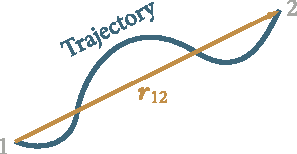
\includegraphics[scale=0.95]{figures/ch_01/fig_1_20.pdf}
			\caption[]{}
			\label{fig:1_20}
		\end{center}
	\end{minipage}
	\hfill{ }%\hspace{-0.1cm}
	\begin{minipage}[t]{0.5\linewidth}
		\begin{center}
			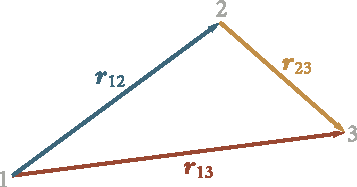
\includegraphics[scale=0.95]{figures/ch_01/fig_1_21.pdf}
			\caption[]{}
			\label{fig:1_21}
		\end{center}
	\end{minipage}
%	\vspace{-0.7cm}
\end{figure}

Assume that a point particle (in the following we shall call it simply a particle for brevity's sake) travelled along a certain trajectory from point $1$ to point $2$ (\fig{1_20}). The path between points $1$ and $2$ measured along the trajectory is called the distance travelled by the particle. We shall denote it by the symbol $s$.

The straight line between points $1$ and $2$, \ie, the shortest distance between these points, is called the displacement of the particle. We shall denote it by the symbol $\vec{r}_{12}$. Let us assume that a particle completes two successive displacements $\vec{r}_{12}$ and $\vec{r}_{23}$ (\fig{1_21}). It is natural to call such a displacement $\vec{r}_{13}$ the sum of the first two that leads to the same result as they do together. Thus, displacements are characterized by magnitude and direction and, besides, are added by using the parallelogram method. Hence, it follows that displacement is a vector.

In everyday life, we use the terms \textbf{speed} and \textbf{velocity} interchangeably, but in physics there is an important distinction between them. Speed depends on the distance travelled, and velocity on the displacement. Speed is the distance travelled by a particle in unit time. If a particle travels identical distances during equal time intervals that may be as small as desired, its motion is called uniform. In this case, the speed of the particle at each moment can be calculated by dividing the distance $s$ by the time $t$.

Velocity is a vector quantity characterizing not only how fast a particle travels along its trajectory, but also the direction in which the particle moves at each moment. Let us divide a trajectory into infinitely small portions of length $\mathrm{d}s$. An infinitely small displacement $\mathrm{d}r$ corresponds to each of these portions (\fig{1_22}). Dividing this displacement by the corresponding time interval $\mathrm{d}t$, we get the instantaneous velocity at the given point of the trajectory:
\begin{equation}\label{eq:1_57}
\vec{v} = \diff{\vec{r}}{t} = \dot{\vec{r}}.
\end{equation}

\noindent
Thus, the velocity is the derivative of the position vector of the particle with respect to time. The displacement $\mathrm{d}r$ coincides with an infinitely small element of the trajectory. Consequently, the vector $\vec{v}$ is directed along a tangent to the trajectory (see \fig{1_22}).

\begin{figure}[t]
	\begin{center}
		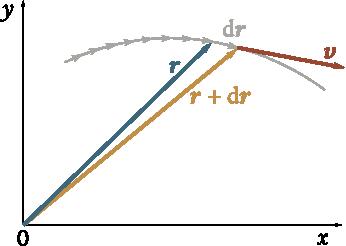
\includegraphics[scale=0.9]{figures/ch_01/fig_1_22.pdf}
		\caption[]{}
		\label{fig:1_22}
	\end{center}
\vspace{-0.7cm}
\end{figure}

Reasoning more strictly, to derive equation~\eqref{eq:1_57} we must proceed as follows.· Having fixed a certain moment of time $t$, let us consider the increment of the position vector $\Delta\vec{r}$ during the small time interval $\Delta t$\footnote{The symbol $\Delta$ (delta) is used in two cases: (a) for designating the increment of a quantity. In the case being considered, $\Delta\vec{r}$ is the increment of the position vector $\vec{r}$ during the time $\Delta t$; (b) for designating a fraction of a quantity. For example, $\Delta t$ is a fraction of the total time $t$ during which motion occurs, and $\Delta s$ is a fraction of the entire 	distance $s$ travelled by the particle.} following $t$ (\fig{1_23}). The ratio $\Delta\vec{r}/\Delta t$ gives the average value of the velocity during the time $\Delta t$. If we take smaller and smaller intervals $\Delta t$, the ratio $\Delta\vec{r}/\Delta t$ in the limit will give us the value of the velocity $\vec{v}$ at the moment $t$:
\begin{equation}\label{eq:1_58}
\vec{v} = \lim_{\Delta t\to 0} \frac{\Delta\vec{r}}{\Delta t} = \diff{\vec{r}}{t}.
\end{equation}

\noindent
We have arrived at equation~\eqref{eq:1_57}.

Let us find the magnitude of the expression~\eqref{eq:1_58}, \ie, the magnitude of the velocity $\vec{v}$:
\begin{equation}\label{eq:1_59}
v = |\vec{v}| = \left|\lim_{\Delta t\to 0} \frac{\Delta\vec{r}}{\Delta t}\right| = \lim_{\Delta t\to 0} \frac{|\Delta\vec{r}|}{\Delta t}.
\end{equation}

\noindent
We cannot write $\Delta r$ instead of $|\Delta\vec{r}|$ in this formula. The vector $\Delta\vec{r}$ is in essence the difference between two vectors ($\vec{r}$ at the moment $t+\Delta t$ minus $\vec{r}$ at the moment $t$). Therefore, its magnitude may be written only with the aid of vertical
bars [see \eqn{1_2}]. The symbol $|\Delta\vec{r}|$ signifies the magnitude of the increment of the vector $\vec{r}$, whereas $\Delta r$ is the increment of the magnitude of the vector $\vec{r}$, \ie, $\Delta|\vec{r}|$. These two quantities, generally speaking, do not equal each other:
\begin{equation*}
|\Delta\vec{r}| \neq \Delta|\vec{r}| = \Delta r.
\end{equation*}

\noindent
The following example will illustrate this. Assume that the vector $\vec{r}$ receives such an increment $\Delta\vec{r}$ that its magnitude does not change, \ie, $|\vec{r}+\Delta\vec{r}|=|\vec{r}|$ (\fig{1_24}). Consequently, the increment of the magnitude of the vector equals zero ($\Delta|\vec{r}| = \Delta r = 0$). At the same time, the magnitude of the increment of the vector $\vec{r}$, \ie, $\Delta|\vec{r}|$, differs from zero (it equals the length of $2-3$). What has been said above holds for any vector $\vec{a}$: in the general case $\Delta|\vec{a}|\neq\Delta|a|$.

\begin{figure}[t]
	\begin{minipage}[t]{0.5\linewidth}
		\begin{center}
			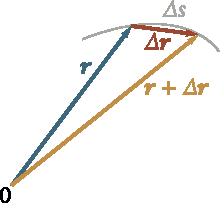
\includegraphics[scale=0.92]{figures/ch_01/fig_1_23.pdf}
			\caption[]{}
			\label{fig:1_23}
		\end{center}
	\end{minipage}
	\hfill{ }%\hspace{-0.1cm}
	\begin{minipage}[t]{0.5\linewidth}
		\begin{center}
			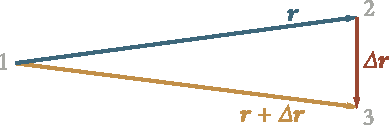
\includegraphics[scale=0.9]{figures/ch_01/fig_1_24.pdf}
			\caption[]{}
			\label{fig:1_24}
		\end{center}
	\end{minipage}
\vspace{-0.7cm}
\end{figure}

Inspection of \fig{1_23} shows that the distance $\Delta s$, generally speaking, differs in value from the magnitude of the displacement $|\Delta\vec{r}|$. If we take increments of the distance $\Delta s$ and the displacement $\Delta\vec{r}$ corresponding to smaller and smaller time intervals $\Delta t$, then the difference between $\Delta s$ and $|\Delta\vec{r}|$ will diminish, and their ratio in the limit will become equal to unity:
\begin{equation*}
\lim_{\Delta t\to 0} \frac{\Delta s}{|\Delta\vec{r}|} = 1.
\end{equation*}

\noindent
On these grounds, we can substitute $\Delta s$ for $|\Delta\vec{r}|$ in equation~\eqref{eq:1_59}, which gives us the expression
\begin{equation}\label{eq:1_60}
v = \lim_{\Delta t\to 0} \frac{\Delta s}{\Delta t} = \diff{s}{t}.
\end{equation}

\noindent
Thus, the magnitude of the velocity equals the derivative of the distance with respect to time.

It is evident that the quantity which in everyday life we call the speed is actually the magnitude of the velocity $\vec{v}$. In uniform motion, the magnitude of the velocity remains constant ($v=\text{constant}$), whereas the direction of the vector $\vec{v}$ changes arbitrarily (in particular it may be constant).

In accordance with \eqn{1_57}, the elementary displacement of a particle is
\begin{equation}\label{eq:1_61}
\mathrm{d}\vec{r} = \vec{v}\,\mathrm{d}{t}.
\end{equation}

\noindent
Sometimes for clarity's sake, we shall denote an elementary displacement by the symbol $\mathrm{d}\vec{s}$, \ie, write \eqn{1_61} in the form
\begin{equation}\label{eq:1_62}
\mathrm{d}\vec{s} = \vec{v}\,\mathrm{d}{t}.
\end{equation}

The velocity vector, like any other vector, can be represented in the form
\begin{equation}\label{eq:1_63}
\vec{v} = v_x\vecuni{x} + v_y\vecuni{y} + v_z\vecuni{z}
\end{equation}

\noindent
where $v_x, v_y, v_z$ are the projections of the vector $\vec{v}$ onto the coordinate axes. At the same time, the vector $\dot{\vec{r}}$ equal to $\vec{v}$, according to \eqn{1_43}, can be written as follows:
\vspace{-12pt}
\begin{equation}\label{eq:1_64}
\dot{\vec{r}} = \dot{x}\vecuni{x} + \dot{y}\vecuni{y} + \dot{z}\vecuni{z}
\end{equation}

\noindent
It follows from a comparison of Eqs.~\eqref{eq:1_63} and~\eqref{eq:1_64} that
\begin{equation}\label{eq:1_65}
v_x = \dot{x},\quad v_y = \dot{y},\quad v_z = \dot{z}.
\end{equation}

\noindent
Consequently, the projection of the velocity vector onto a coordinate axis equals the time derivative of the relevant coordinate of the moving particle. Taking Eq. \eqref{eq:1_10} into account, we get:
\begin{equation}\label{eq:1_66}
v = \sqrt{\dot{x}^2 + \dot{y}^2 + \dot{z}^2}.
\end{equation}

The velocity vector can be written in the form $\vec{v}=v\vecuni{v}$, where $v$ is the magnitude of the velocity, and $\vecuni{v}$ is the unit vector of $\vec{v}$. Let us introduce the unit vector $\hatvec{\tau}$ of the tangent to a trajectory with its sense the same as that of $\vec{v}$. Hence, obviously, the unit vectors $\vecuni{v}$ and $\hatvec{\tau}$ will coincide, and we can write the following expression:
\vspace{-12pt}
\begin{equation}\label{eq:1_67}
\vec{v} = v\vecuni{v} = v\hatvec{\tau}.
\end{equation}

Let us obtain still another expression for $\vec{v}$. For this purpose, we shall introduce the position vector in the form of $\vec{r}=r\vecuni{r}$ into \eqn{1_57}. According to \eqn{1_49}, we have
\begin{equation}\label{eq:1_68}
\vec{v} = \dot{\vec{r}} = \dot{r}\vecuni{r} + r\dot{\hat{\boldsymbol{e}}}_r.
\end{equation}

\noindent
We shall limit ourselves, for simplicity, to the case when the trajectory is a plane curve, \ie, a curve such that all its points are in a single plane. Let this plane be the plane $x, y$. In \eqn{1_68}, the vector $\vec{v}$ written in the form of two components (\fig{1_25}). The first of them, which we shall designate $\vec{v}_r$, is
\begin{equation}\label{eq:1_69}
\vec{v}_r = \dot{r}\vecuni{r}.
\end{equation}

\noindent
It is directed along the position vector $\vec{r}$ and characterizes the rate of change of the magnitude of $\vec{r}$. The second component, which we shall designate $\vec{v}_{\varphi}$, is
\begin{equation}\label{eq:1_70}
\vec{v}_{\varphi} = r\dot{\hat{\boldsymbol{e}}}_r.
\end{equation}

\noindent
It characterizes the rate of change of the direction of the position vector.

\begin{figure}[t]
	\begin{center}
		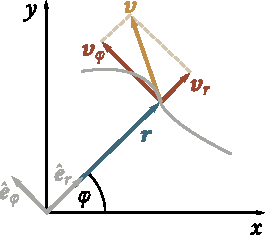
\includegraphics[scale=1]{figures/ch_01/fig_1_25.pdf}
		\caption[]{}
		\label{fig:1_25}
	\end{center}
	\vspace{-0.7cm}
\end{figure}

Using \eqn{1_56}, we can write that
\begin{equation*}
\dot{\hat{\boldsymbol{e}}}_r = \diff{\varphi}{t}\vecuni{\varphi} = \dot{\varphi}\vecuni{\varphi}
\end{equation*}

\noindent
where $\varphi$ is the angle between the position vector and the $x$-axis, and $\vecuni{\varphi}$ is a unit vector perpendicular to the position vector with its sense in the direction of growth of the angle $\varphi$ [in \eqn{1_56} the symbol $\vecuni{\perp}$ was used for this unit vector]. Using this value in \eqn{1_70}, we get:
\begin{equation}\label{eq:1_71}
\vec{v}_{\varphi} = r\dot{\varphi}\vecuni{\varphi}.
\end{equation}

\noindent
We have introduced the symbols $\vec{v}_{\varphi}$ and $\vecuni{\varphi}$ to underline the fact that the component $\vec{v}_{\varphi}$ and the corresponding unit vector are related to a change in the angle $\varphi$.

The vectors $\vec{v}_r$ and $\vec{v}_{\varphi}$ are obviously mutually perpendicular. Hence,
\begin{equation}\label{eq:1_72}
v = \sqrt{v_r^2 + v_{\varphi}^2} = \sqrt{\dot{r}^2 + r^2\dot{\varphi}^2}.
\end{equation}

Now let us consider how to calculate the distance travelled by a particle from the moment of time $t_1$ to $t_2$ if we know the speed at each moment. Let us divide the interval $t_2-t_1$ into $N$ small, but not necessarily equal intervals: $\Delta t_1$, $\Delta t_2$, \ldots, $\Delta t_N$. The total distance $s$ travelled by a particle can be represented as the sum of the distances $\Delta s_1$, $\Delta s_2$, \ldots, $\Delta s_N$ travelled during the relevant time intervals $\Delta t$:
\begin{equation*}
s = \Delta s_1 + \Delta s_2 + \ldots + \Delta s_N = \sum_{i=1}^{N} \Delta s_i.
\end{equation*}

\noindent
In accordance with \eqn{1_60}, each of the addends can approximately be represented in the form
\begin{equation*}
\Delta s_i \approx v_i \Delta t_i
\end{equation*}

\noindent
where $\Delta t_i$ is the time interval during which the distance $\Delta s_i$ was travelled, and $v_i$ is one of the values of the speed during the time $\Delta t_i$. Hence,
\begin{equation}\label{eq:1_73}
s \approx \sum_{i=1}^{N} v_i \Delta t_i.
\end{equation}

\noindent
This expression will be obeyed more accurately with diminishing time intervals $\Delta t_i$. In the limit when all the $\Delta t_i$'s tend to zero (the number of intervals $\Delta t_i$ will correspondingly grow unlimitedly), the approximate equation will become accurate:
\begin{equation*}
s = \lim_{\Delta t_i\to 0} \sum_{i=1}^{N} v_i \Delta t_i.
\end{equation*}

This expression is a definite integral of the function $v(t)$ taken within the limits from $t_1$ to $t_2$. Thus, the distance travelled by a particle during the interval from $t_1$ to $t_2$ is
\begin{equation}\label{eq:1_74}
s = \int_{t_1}^{t_2} v(t)\,\mathrm{d}t.
\end{equation}

\noindent
It must be underlined that here we are speaking of the speed. If we take an integral of the velocity $\vec{v}(t)$, we get the vector of the displacement of the particle from the point where it was at the moment $t_1$ to the point where it was at the moment $t_2$:
\begin{equation}\label{eq:1_75}
\int_{t_1}^{t_2} v(t)\,\mathrm{d}t = \int_{t_1}^{t_2} \mathrm{d}\vec{r} = \vec{r}_{12}
\end{equation}

\noindent
[see \eqn{1_61}].

If we plot the dependence of $v$ on $t$ (\fig{1_26}), then the distance travelled can be represented as the area of the figure confined between the curve $v(t)$, the straight lines $t = t_1$ and $t = t_2$, and the $t$-axis. Indeed, the product $v_i\Delta t_i$ numerically equals the area of the $i$-th strip. The sum \eqn{1_73} equals the area of the figure confined on top by the broken line formed by the top edges of all such strips. When all the $\Delta t_i$'s tend to zero, the width of a strip diminishes (their number grows simultaneously), and the broken line will coincide with the curve $v = v(t)$ in the limit. Thus, the distance travelled during the time from the moment $t_1$ to the moment $t_2$ numerically equals the area confined between the curve of the function $v = v(t)$, the time axis, and the straight lines $t = t_1$ and $t = t_2$.

\begin{figure}[t]
	\begin{center}
		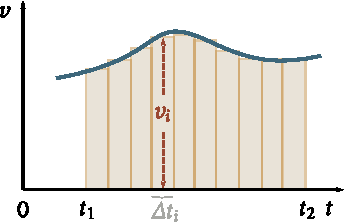
\includegraphics[scale=1]{figures/ch_01/fig_1_26.pdf}
		\caption[]{}
		\label{fig:1_26}
	\end{center}
	\vspace{-0.8cm}
\end{figure}

It should be noted that the average value of the speed during
the time from $t = t_1$ to $t = t_2$, by definition, is
\begin{equation*}
\average{v} = \frac{s}{t_2-t_1}.
\end{equation*}

\noindent
(The symbol $\langle\rangle$ embracing the $v$ indicates an average.) Introducing into this equation the expression~\eqref{eq:1_74} for $s$, we get
\begin{equation}\label{eq:1_76}
\average{v} = \frac{1}{t_2-t_1}\,\int_{t_1}^{t_2}v(t)\,\mathrm{d}t.
\end{equation}

\noindent
The average values of any scalar or vector functions are calculated in a similar way. For example, the average value of the velocity is
\begin{equation}\label{eq:1_77}
\average{\vec{v}} = \frac{1}{t_2-t_1}\,\int_{t_1}^{t_2}\vec{v}(t)\,\mathrm{d}t = \frac{\vec{r}_{12}}{t_2-t_1}.
\end{equation}

\noindent
[see \eqn{1_75}]. The average value of the function $y(x)$ within the interval from $x_1$ to $x_2$ is determined by the expression
\begin{equation}\label{eq:1_78}
\average{y} = \frac{1}{t_2-t_1}\,\int_{x_1}^{x_2}y(t)\,\mathrm{d}x.
\end{equation}

\section{Acceleration}\label{sec:1_4}

The velocity $\vec{v}$ of a particle can change with time both in magnitude and in direction. The rate of change of the vector $\vec{v}$, like the rate of change of any function of time, is determined by the derivative of the vector $\vec{v}$ with respect to $t$. Denoting this derivative by the symbol $\vec{a}$, we get:
\begin{equation}\label{eq:1_79}
\vec{a} = \lim_{\Delta t\to 0}\frac{\Delta\vec{v}}{\Delta t} = \diff{\vec{v}}{t} = \dot{\vec{v}}.
\end{equation}

\noindent
The quantity determined by equation~\eqref{eq:1_79} is called the \textbf{acceleration} of the particle.

It must be noted that the acceleration $\vec{a}$ plays the same part with respect to $\vec{v}$ as the vector $\vec{v}$ does with respect to the position vector $\vec{r}$.

Equal vectors have identical projections onto the coordinate axes. Consequent-ly, for example,
\begin{equation*}
a_x = \left(\diff{\vec{v}}{t}\right)_{\text{pr. }\vec{x}} = \diff{v_x}{t} = \dot{v}_x
\end{equation*}

\noindent
[see Eqs.~\eqref{eq:1_40}]. At the same time according to Eqs.~\eqref{eq:1_65}, we have $v_x=\dot{x}=\diffin{x}{t}$. Therefore,
\begin{equation*}
\diff{v_x}{t} = \frac{\mathrm{d}}{\mathrm{d}t} \left(\diff{x}{t}\right) = \diffsec{x}{t} = \ddot{x}.
\end{equation*}

\noindent
What we have obtained is that the projection of the acceleration vector onto the $x$-axis equals the second derivative of the coordinate $x$ with respect to time: $a_x=\ddot{x}$. Similar expressions are obtained for the projections of the acceleration onto the $y$- and $z$-axes. Thus,
\begin{equation}\label{eq:1_80}
a_x=\ddot{x},\quad a_y=\ddot{y},\quad a_z=\ddot{z}.
\end{equation}

Using \eqn{1_67} for $\vec{v}$ in~\eqref{eq:1_79}, we get:
\begin{equation}\label{eq:1_81}
\vec{a} = \diff{(v\hatvec{\tau})}{t}.
\end{equation}

\noindent
We remind our reader that $\hatvec{\tau}$ is the unit vector of a tangent to a trajectory having the same direction as $\vec{v}$. According to \eqn{1_49},
\begin{equation}\label{eq:1_82}
\vec{a} = \dot{v}\hatvec{\tau} + v\dot{\hatvec{\tau}}.
\end{equation}

\noindent
Hence, the vector $\vec{a}$ can be represented in the form of the sum of two components. One of them has the direction $\hatvec{\tau}$, \ie, is tangent to the trajectory. It is therefore designated $\vec{a}_{\hatvec{\tau}}$ and is called the \textbf{tangential acceleration}. It equals
\begin{equation}\label{eq:1_83}
\vec{a}_{\hatvec{\tau}} = \dot{v}\hatvec{\tau}.
\end{equation}

\noindent
The second component equal to $v\dot{\hatvec{\tau}}$ is directed, as we shall show below, along a normal to the trajectory. It is therefore designated $\vec{a}_{\hatvec{n}}$ and is called the \textbf{normal acceleration}. Thus,
\begin{equation}\label{eq:1_84}
\vec{a}_{\hatvec{n}} = v\dot{\hatvec{\tau}}.
\end{equation}

In studying the properties of the two components, we shall restrict ourselves for the sake of simplicity to the case when the trajectory is a plane curve.

The magnitude of the tangential acceleration~\eqref{eq:1_83} is
\begin{equation}\label{eq:1_85}
\vec{a}_{\hatvec{\tau}} = |\dot{v}|.
\end{equation}

\noindent
If $\dot{v}>0$ (the velocity grows in magnitude), then the vector $\vec{a}_{\hatvec{\tau}}$ has the same direction as $\hatvec{\tau}$ (\ie, the same direction as $\vec{v}$). If $\dot{v}<0$ (the velocity decreases with time), then the vectors $\vec{v}$ and $\vec{a}_{\hatvec{\tau}}$ have opposite directions. In uniform motion, $\dot{v}=0$, and, therefore, tangential acceleration is absent.

To determine the properties of the normal acceleration [\eqn{1_84}], we must find out what $\dot{\hatvec{\tau}}$, \ie, the rate of change with time of the direction of a tangent to the trajectory, is determined by. It is easy to understand that this rate will grow with an increasing curvature of the trajectory and a higher velocity of a particle along it.

The degree of bending of a plane curve is characterized by its curvature $C$ determined by the expression
\begin{equation}\label{eq:1_86}
C = \lim_{\Delta t\to 0} \frac{\Delta\varphi}{\Delta s} = \diff{\varphi}{s}
\end{equation}

\noindent
where $\Delta\varphi$ is the angle between tangents to the curve at points spaced $\Delta s$ apart (\fig{1_27}). Thus, the curvature determines the rate of turning of a tangent in motion along a curve.

\begin{figure}[t]
	\begin{center}
		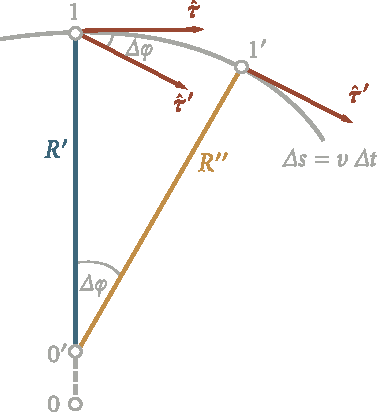
\includegraphics[scale=1]{figures/ch_01/fig_1_27.pdf}
		\caption[]{}
		\label{fig:1_27}
	\end{center}
	\vspace{-0.7cm}
\end{figure}


The reciprocal of the curvature $C$ is called the \textbf{radius of curvature} at the given point of the curve and is designated $R$:
The degree of bending of a plane curve is characterized by its curvature $C$ determined by the expression
\begin{equation}\label{eq:1_87}
R = \frac{1}{C} = \lim_{\Delta\varphi\to 0} \frac{\Delta s}{\Delta\varphi} = \diff{s}{\varphi}.
\end{equation}

\noindent
The radius of curvature is the radius of a circle that coincides at the given spot with the curve on an infinitely small portion of it. The centre of this circle is defined as the centre of curvature for the given point of the curve.

The radius and centre of curvature at point $1$ (see \fig{1_27}) can be determined as follows. Take point $1'$ near point $1$. Draw the tangents $\hatvec{\tau}$ and $\hatvec{\tau}'$ at these points. The perpendiculars to the tangents will intersect at a certain point $0'$. We must note that for a curve which is not a circle the distances $R'$ and $R''$ will differ somewhat from each other. If point $1'$ is brought closer to point $1$, the point of intersection $0'$ of the perpendiculars will move along the straight line $R'$ and in the limit will be at point $0$. It is exactly the latter that will be the centre of curvature for point $1$. The distances $R'$ and $R"$ will tend to a common limit $R$ equal to the radius of curvature. Indeed, if points $1$ and $1'$ are close to each other, we can write that $\Delta\varphi\approx\Delta s/R'$ or $R' \approx \Delta s/\Delta\varphi$. In the limit when $\Delta\varphi\to 0$, this approximate equation will transform into the strict equation $R=\diffin{s}{\varphi}$ coinciding with the definition of the radius of curvature [see \eqn{1_87}].

Let us now turn to the calculation of an [see \eqn{1_84}]. According to \eqn{1_56},
\begin{equation}\label{eq:1_88}
\dot{\hatvec{\tau}} = \diff{\varphi}{t}\hatvec{n}
\end{equation}

\noindent
where $\hatvec{n}$ is the unit vector of the normal to the trajectory with its sense in the direction of rotation of the vector $\hatvec{\tau}$ when a particle travels along the trajectory [in \eqn{1_56} a similar unit vector was designated $\vecuni{\perp}$]. The quantity $\diffin{\varphi}{t}$ can be related to the radius of curvature of the trajectory and the speed of the particle $\vec{v}$. It follows from \fig{1_27} that
\begin{equation*}
\Delta\varphi\approx \frac{\Delta s}{R'} = \frac{v'\,\Delta t}{R'}
\end{equation*}

\noindent
where $\Delta\varphi$ is the angle of rotation of the vector $\hatvec{\tau}$ during the time $\Delta t$ (coinciding with the angle between the perpendiculars $R'$ and $R''$), and $v'$ is the average speed over the distance $\Delta s$. Hence,
\begin{equation*}
\frac{\Delta\varphi}{\Delta s} \approx \frac{v'}{R'}.
\end{equation*}

\noindent
In the limit when $\Delta t$ tends to zero, the approximate equation will become a strict one, the average speed $v'$ will transform into the instantaneous speed $v$ at point $1$, and $R'$ will become the radius of curvature $R$. As a result, we get the equation
\begin{equation}\label{eq:1_89}
\diff{\varphi}{t} = \frac{v}{R} = vC
\end{equation}

\noindent
($C$ is the curvature). Hence, the rate of rotation of the velocity vector, as we assumed, is proportional to the curvature of the trajectory and the speed of a particle along its trajectory.

Using \eqn{1_89} in~\eqref{eq:1_88}, we find that $\dot{\hatvec{\tau}}=(v/R)\hatvec{n}$. And at last, introducing this expression into \eqn{1_84}, we arrive at the final equation for the normal acceleration:
\vspace{-12pt}
\begin{equation}\label{eq:1_90}
\vec{a}_{\hatvec{n}} = \diff{v^2}{R}\hatvec{n}.
\end{equation}

Thus, the acceleration vector when a particle travels along a plane curve is determined by the following expression:
\begin{equation}\label{eq:1_91}
\vec{a} = \vec{a}_{\hatvec{\tau}} + \vec{a}_{\hatvec{n}} = \dot{v}\hatvec{\tau} + \frac{v^2}{R}\hatvec{n}.
\end{equation}

\noindent
The magnitude of the vector $\vec{a}$ is
\begin{equation}\label{eq:1_92}
a = \sqrt{a_{\hatvec{\tau}}^2 + a_{\hatvec{n}}^2} = \sqrt{\dot{v}^2 + \left(\frac{v^2}{R}\right)^2}.
\end{equation}

In rectilinear motion, the normal acceleration is absent. It must be noted that an vanishes at the inflection point of a curvilinear trajectory (at point IP in \fig{1_28}). At both sides of this point, the vectors $\vec{a}_{\hatvec{n}}$ have different directions. The vector $\vec{a}_{\hatvec{n}}$ cannot change in a jump. Its direction reverses smoothly, and it becomes equal to zero at the inflection point. Assume that a particle is travelling uniformly with an acceleration constant in magnitude. Since in uniform motion the magnitude of the velocity does not change, we have $\vec{a}_{\hatvec{\tau}}=0$, so that $\vec{a}=\vec{a}_{\hatvec{n}}$. The constant magnitude of an signifies that $v^2/R=\text{constant}$. Hence, we conclude that $R=\text{constant}$ ($v=\text{constant}$ because the motion is uniform). This means that the particle is travelling along a curve of constant curvature, \ie, a circle. Thus, when the acceleration of a particle is constant in magnitude and is directed at each moment of time at right angles to the velocity vector, the trajectory of the particle will be a circle.

\begin{figure}[t]
	\begin{center}
		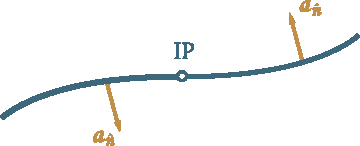
\includegraphics[scale=0.95]{figures/ch_01/fig_1_28.pdf}
		\caption[]{}
		\label{fig:1_28}
	\end{center}
	\vspace{-0.6cm}
\end{figure}

%\begin{figure}[t]
%	\begin{minipage}[t]{0.5\linewidth}
%		\begin{center}
%			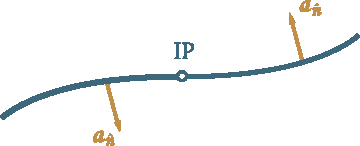
\includegraphics[scale=0.95]{figures/ch_01/fig_1_28.pdf}
%			\caption[]{}
%			\label{fig:1_28}
%		\end{center}
%	\end{minipage}
%	\hfill{ }%\hspace{-0.1cm}
%	\begin{minipage}[t]{0.5\linewidth}
%		\begin{center}
%			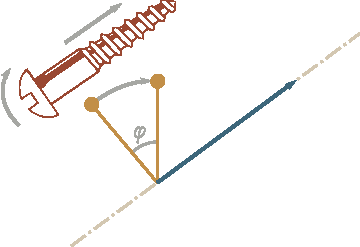
\includegraphics[scale=0.95]{figures/ch_01/fig_1_29.pdf}
%			\caption[]{}
%			\label{fig:1_29}
%		\end{center}
%	\end{minipage}
%	\vspace{-0.4cm}
%\end{figure}

\section{Circular Motion}\label{sec:1_5}

The rotation of a body through a certain angle $\varphi$ can be given in the form of a straight line whose length is $\varphi$ and whose direction coincides with the axis about which the body is rotating. To indicate the direction of rotation about a given axis, it is related to the line depicting rotation by the \textbf{right-hand screw rule}: the line should be directed so that when looking along it (\fig{1_29}) we see clockwise rotation (when rotating the head of a right-hand screw clockwise, we cause it to move away from us). We showed in Sec.~\ref{sec:1_2} (see \fig{1_4}) that rotations through finite angles are not added by the parallelogram method and are therefore not vectors. Matters are different for rotations through very small angles $\Delta\vec{\varphi}$. The distance travelled by any point of a body when rotated through a very small angle can be considered as a straight line (\fig{1_30}). Consequently, two small circular motions $\Delta\vec{\varphi}_1$ and $\Delta\vec{\varphi}_2$ performed sequentially, as can be seen from the figure, result in the same displacement $\Delta\vec{r}_3=\Delta\vec{r}_1+\Delta\vec{r}_2$ of any point of the body as the circular motion $\Delta\vec{\varphi}_3$ obtained from $\Delta\vec{\varphi}_1$ and $\Delta\vec{\varphi}_2$ by addition using the parallelogram method. Hence it follows that very small circular motions can be considered as vectors (we shall denote these vectors by $\Delta\vec{\varphi}$ or $\mathrm{d}\vec{\varphi}$). The direction of the rotation vector is associated with the direction of rotation of a body. Consequently, $\mathrm{d}\vec{\varphi}$ is not a true vector, but a pseudovector.

\begin{figure}[t]
	\begin{center}
		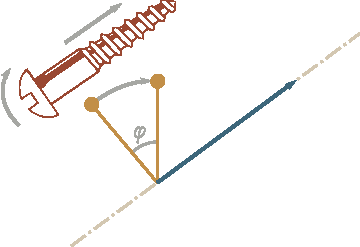
\includegraphics[scale=0.95]{figures/ch_01/fig_1_29.pdf}
		\caption[]{}
		\label{fig:1_29}
	\end{center}
	\vspace{-0.7cm}
\end{figure}

The vector quantity
\begin{equation}\label{eq:1_93}
\vec{\omega} = \lim_{\Delta t\to 0} \frac{\Delta\vec{\varphi}}{\Delta t} = \diff{\vec{\varphi}}{t}
\end{equation}

\noindent
(where $\Delta t$ is the time during which the circular motion $\Delta\vec{\varphi}$ is performed) is called the angular velocity of a body\footnote{The velocity $\vec{v}$ considered in Sec.~\ref{sec:1_3} is sometimes called linear.}. The angular velocity $\vec{\omega}$ is directed along the axis about which the body is rotating in a direction determined by the right-hand screw rule (\fig{1_31}) and is a pseudovector. The magnitude of the angular velocity, \ie, the angular speed, equals $\diffin{\varphi}{t}$. Circular motion at a constant angular velocity is called uniform. For uniform circular motion, we have $\omega=\varphi t$, where $\varphi$ is the finite angle of rotation during the time $t$ (compare with $v=s/t$). Thus, in uniform circular motion, $\omega$ shows the angle through which a body rotates in unit time.

\begin{figure}[t]
	\begin{minipage}[t]{0.5\linewidth}
		\begin{center}
			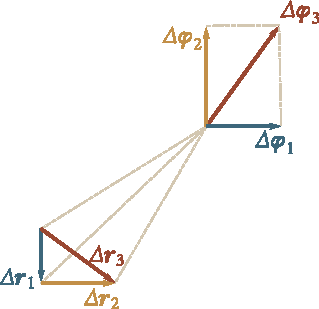
\includegraphics[scale=1]{figures/ch_01/fig_1_30.pdf}
			\caption[]{}
			\label{fig:1_30}
		\end{center}
	\end{minipage}
	\hspace{-0.1cm}
	\begin{minipage}[t]{0.5\linewidth}
		\begin{center}
			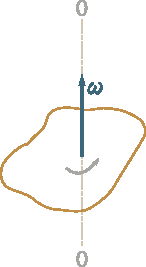
\includegraphics[scale=0.95]{figures/ch_01/fig_1_31.pdf}
			\caption[]{}
			\label{fig:1_31}
		\end{center}
	\end{minipage}
	\vspace{-0.5cm}
\end{figure}

Uniform circular motion can be characterized by the \textbf{period of revolution} $T$. It is defined as the time  during which a body completes one revolution, i.e. rotates through the angle \SI{2\pi}{\radian}, or \SI{360}{\degree}. Since the time interval $\Delta t=T$ corresponds to the angle of rotation $\Delta\varphi=2\pi$, we have
\begin{equation}\label{eq:1_94}
\omega = \frac{2\pi}{T}
\end{equation}

\noindent
whence
\begin{equation}\label{eq:1_95}
T = \frac{2\pi}{\omega}.
\end{equation}

The number of revolutions in unit time $\nu$ is evidently equal to
\begin{equation}\label{eq:1_96}
\nu = \frac{1}{T} = \frac{\omega}{2\pi}.
\end{equation}

\noindent
It follows from \eqn{1_96} that the angular velocity equals $2\pi$ multiplied by the number of revolutions per unit time:
\begin{equation}\label{eq:1_97}
\omega = 2\pi\nu.
\end{equation}

The concepts of the period of revolution and the number of revolutions per unit time can also be retained for non-uniform circular motion. Here, we must understand the instantaneous value of $T$ to signify the time during which a body would perform one revolution if it rotated uniformly with the given instantaneous value of the angular velocity, and $\nu$ to signify the number of revolutions which a body would complete in unit time in similar conditions.

The vector $\vec{\omega}$ may vary either as a result of a change in the speed of rotation of a body about its axis (in this case it changes in magnitude), or as a result of turning of the axis of rotation in space (in this case $\vec{\omega}$ changes in direction). Assume that during the time $\Delta t$ the vector $\vec{\omega}$ receives the increment $\Delta\vec{\omega}$. The change in the angular velocity vector with time is characterized by the quantity
\begin{equation}\label{eq:1_98}
\vec{\alpha} = \lim_{\Delta t\to 0} \frac{\Delta\vec{\omega}}{t} = \diff{\vec{\omega}}{t}
\end{equation}

\noindent
called the \textbf{angular acceleration}. The latter, like the angular velocity, is a pseudovector.

%\begin{figure}[t]
%	\begin{center}
%		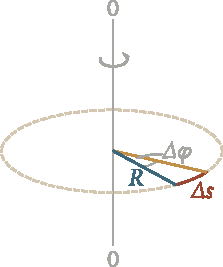
\includegraphics[scale=1]{figures/ch_01/fig_1_32.pdf}
%		\caption[]{}
%		\label{fig:1_32}
%	\end{center}
%\vspace{-0.7cm}
%\end{figure}
\begin{figure}[t]
	\begin{minipage}[t]{0.5\linewidth}
		\begin{center}
			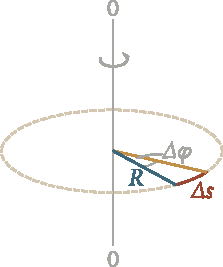
\includegraphics[scale=1]{figures/ch_01/fig_1_32.pdf}
			\caption[]{}
			\label{fig:1_32}
		\end{center}
	\end{minipage}
	\hspace{-0.1cm}
	\begin{minipage}[t]{0.5\linewidth}
		\begin{center}
			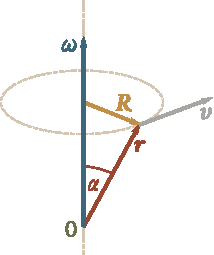
\includegraphics[scale=1]{figures/ch_01/fig_1_33.pdf}
			\caption[]{}
			\label{fig:1_33}
		\end{center}
	\end{minipage}
	\vspace{-0.6cm}
\end{figure}

Different points of a body in circular motion have different linear velocities $\vec{v}$. The velocity of each point continuously changes its direction. The speed $v$ is determined by the speed of rotation of the body $\omega$ and the distance $R$ to the point being considered from the axis of rotation. Assume that during a small interval of time the body turned through the angle $\Delta\varphi$ (\fig{1_32}). The point at the distance $R$ from the axis travels the path $\Delta s=R\Delta\varphi$. The linear speed of the point is
\begin{equation*}
v = \lim_{\Delta t\to 0} \frac{\Delta s}{\Delta t} = \lim_{\Delta t\to 0} R\frac{\Delta\varphi}{\Delta t} = R \lim_{\Delta t\to 0} \frac{\Delta\varphi}{\Delta t} = R\diff{\varphi}{t} = R\omega.
\end{equation*}

\noindent
Thus,
\begin{equation}\label{eq:1_99}
v = \omega R.
\end{equation}

Equation~\eqref{eq:1_99} relates the linear and the angular speeds. Let us find an expression relating the relevant velocities $\vec{v}$ and $\vec{\omega}$. We shall determine the position of the point of the body being considered by the position vector $\vec{r}$ drawn from the origin of coordinates on the axis of rotation (\fig{1_33}). Examination of the figure shows that the vector product $\vecprod{\omega}{r}$ coincides in direction with the vector $\vec{v}$ and its magnitude is $\omega r\sin\alpha=\omega R$. Hence,
\begin{equation}\label{eq:1_100}
\vec{v} = \vecprod{\omega}{r}.
\end{equation}

%\begin{figure}[t]
%	\begin{center}
%		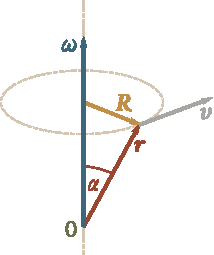
\includegraphics[scale=1]{figures/ch_01/fig_1_33.pdf}
%		\caption[]{}
%		\label{fig:1_33}
%	\end{center}
%	\vspace{-0.7cm}
%\end{figure}

The normal acceleration of the points of a rotating body is $\vec{a}_{\hatvec{n}}=v^2/R$. Introducing into this expression the value of $v$ from \eqn{1_99}, we get
\begin{equation}\label{eq:1_101}
a_{\hatvec{n}} = \omega^2 R.
\end{equation}

\noindent
If we introduce the vector $\vec{R}$ drawn to the given point of the body from the axis of rotation at right angles to the latter (see \fig{1_33}), then \eqn{1_101} can be given a vector form:
\begin{equation}\label{eq:1_102}
\vec{a}_{\hatvec{n}} = -\omega^2 \vec{R}.
\end{equation}

\noindent
There is a minus sign in this formula because the vectors $\vec{a}_{\hatvec{n}}$ and $\vec{R}$ have opposite directions.

Let us assume that the axis of rotation of a body does not turn in space. According to \eqn{1_85}, the magnitude of the tangential acceleration is $|\diffin{v}{t}|$. Using equation~\eqref{eq:1_99} and taking into account that the distance to the point being considered from the axis of rotation $R=\text{constant}$, we can write
\begin{equation*}
a_{\hatvec{\tau}} = \left| \lim_{\Delta t\to 0} \frac{\Delta v}{\Delta t} \right| = \left| \lim_{\Delta t\to 0} \frac{\Delta(\omega R)}{\Delta t} \right| = R \left| \lim_{\Delta t\to 0} \frac{\Delta(\omega)}{\Delta t} \right| = R\alpha
\end{equation*}

\noindent
where $\alpha$, is the magnitude of the angular acceleration. Consequently, the magnitude of the tangential acceleration is related to the magnitude of the angular acceleration as follows:
\begin{equation}\label{eq:1_103}
a_{\hatvec{\tau}} = \alpha R.
\end{equation}

Thus, the normal and tangential accelerations grow linearly with an increasing distance to a point from the axis of rotation.
